\graphicspath{{img/capture_intro/}}
%%%%%%%%%%%%%%%%%%%%%%%%%%%%%%%%%%%%%
%%%%%%%%%%%%%%%%%%%%%%%%%%%%%%%%%%%%%
%%%%%%%%%%%%%%%%%%%%%%%%%%%%%%%%%%%%%

\chapter{Improved Treatment of Dark Matter Capture in Compact Objects}
\label{chapter:capture_intro}

\begin{synopsis}
This chapter combines aspects of Refs.~\cite{Bell:2020jou_sep_ImprovedTreatmentDark,Bell:2020lmm_mar_ImprovedTreatmentDark,Anzuini:2021lnv_nov_Improvedtreatmentdark} to give a complete introduction to the formalism we have built for dark matter capture in compact objects. We begin by reviewing aspects of Gould's formalism for capture in the Sun~\cite{Gould:1987ir_ResonantEnhancementsWIMP,Gould:1987ju_WeaklyInteractingMassive}. We then build upon these results to incorporate relativistic corrections and the effects of Pauli Blocking due to scattering from a degenerate media in a self-consistent manner. Important aspects of both the interaction and capture rates are discussed, including Pauli blocking for low mass DM and the effects of multiple scatting in the high-mass regime. We then apply our results to the example DM scattering from neutron targets using the BSk24 EoS to model the neutron star.
\end{synopsis}
%%%%%%%%%%%%%%%%%%%%%%%%%%%%%%%%%%%%%
%%%%%%%%%%%%%%%%%%%%%%%%%%%%%%%%%%%%%
%%%%%%%%%%%%%%%%%%%%%%%%%%%%%%%%%%%%%



%%%%%%%%%%%%%%%%%%%%%%%%%%%%%%%%%%%%%
%%%%%%%%%%%%%%%%%%%%%%%%%%%%%%%%%%%%%
%%%%%%%%%%%%%%%%%%%%%%%%%%%%%%%%%%%%%
\section{Dark Matter Capture in the Sun}
\label{ch3:sec:solar_capture_full}
%%%%%%%%%%%%%%%%%%%%%%%%%%%%%%%%%%%%%
%%%%%%%%%%%%%%%%%%%%%%%%%%%%%%%%%%%%%
%%%%%%%%%%%%%%%%%%%%%%%%%%%%%%%%%%%%%

Before jumping into the capture formalism relevant to compact objects, it will serve us well to review the formalism laid out by Gould for capture in the Sun~\cite{Gould:1987ju_WeaklyInteractingMassive, Gould:1987ir_ResonantEnhancementsWIMP}. 

To begin, we consider the flux of dark matter particles that pass through a spherical shell a large distance $R$ from the star, where the gravitational field is negligible. For this, we need to know the distribution function of the relative velocity between the DM and the stellar constituents. 
The velocity distribution function will be spatially isotropic, and so for simplicity we will assume that the DM follows a Maxwell-Boltzmann distribution function, 
\begin{equation}
    f_\infty(\tilde{u}_\chi) d\tilde{u}_\chi= 4 \pi \left( \frac{3}{2 \pi} \right)^{3/2}\frac{\tilde{u}_\chi^2}{v_d^2} \exp\left(-\frac{3 \tilde u_\chi^2}{2 v_d^3}\right)\,d\tilde u_\chi, 
\end{equation}
where $\tilde u_\chi$ is the DM velocity in the halo, and $v_d$ is the DM halo velocity dispersion.

Taking into account the motion of the star through the halo and the thermal motion of the constituents, which are assumed to follow a Maxwell-Boltzmann distribution, gives the relative velocity between the DM and targets, $ u_\chi$. 
The distribution function for the relative velocity can be expressed as~\cite{Busoni:2017mhe_oct_Evaporationscatteringmomentum}
\begin{equation}
    f_{\mathrm{MB}}(u_\chi, \Tstar)du_\chi = \frac{u_\chi}{v_\star} \sqrt{\frac{3 }{2 \pi (v_d^2 + 3 T_\star /\mi)}} \left( e^{-\frac{3(u_\chi - v_\star)^2}{2(v_d^2 + 3 T_\star /\mi)}} - e^{-\frac{3(u_\chi + v_\star)^2}{2(v_d^2 + 3 T_\star /\mi)}} \right)du_\chi,
    \label{ch3:eq:MB_finit_T}
\end{equation}
where $v_\star$ is the star's velocity in the halo rest frame\footnote{This is the frame where the DM has an average velocity of zero.}, $T_\star$ is the temperature of the star, and $\mi$ is the mass of the target.

Returning to the large spherical shell of radius $R$, given the velocity distribution function, we can obtain the flux of DM through this surface. The rate of DM particles passing through a surface element $d\tilde{A}$ with velocity between $u_\chi$ and $u_\chi + du_\chi$, with an angle to the normal of $d\tilde{A}$ between $\tilde\theta$ and $\tilde \theta + d\tilde \theta$ and an azimuthal angle between $\tilde \phi$ and $\tilde \phi + d\tilde \phi$ is given by~\cite{Press:1985ug_Capturesungalactic}
\begin{align}
    \frac{dN_\chi}{dt} &= \frac{\rho_\chi}{m_\chi}f_{\mathrm{MB}}(u_\chi, \Tstar) \vec{u}\cdot d\vec{\tilde{A}}\, d u_\chi\, \frac{d\tilde \Omega}{4\pi}\\
    & = \frac{\rho_\chi}{m_\chi}\fMB(u_\chi, \Tstar)u_\chi \cos\tilde\theta \,d\tilde{A}\, d u_\chi\,  \frac{d\cos\tilde\theta \,d\tilde\phi}{4\pi}\\
    & = \frac{1}{4}\frac{\rho_\chi}{m_\chi}\fMB(u_\chi, \Tstar)u_\chi d\tilde{A}\, d u_\chi\,d\cos^2\tilde\theta,
\end{align}
where we have integrated over the azimuthal angle $\tilde \phi$ due to the isotropy of the system. The number density of the DM is included through the $\rho_\chi/m_\chi$ factor. 
Integrating over the area of the sphere is trivial due to isotropy, leaving us with 
\begin{align}
    \frac{dN_\chi}{dt} &= \pi \frac{\rho_\chi}{m_\chi} f(u_\chi, \Tstar)u_\chi\, d u_\chi \, d\cos^2\tilde\theta,
\end{align}
with the integration interval for $\cos^2\tilde\theta$ being $(0, 1)$.

As the DM begins to infall from this large distance $R$ to a closer distance $r$, the star's gravitational field will boost the velocity by the local escape velocity $v_e(r)$ such that
\begin{align}
    w^2_\chi(r) &= u^2_\chi + v_e^2(r),\\
    v_e^2(r) & = \frac{2 G M_\star}{R_\star} + \int_r^{R_\star} \frac{G M_\star(r')}{r'^2}\,dr'.
\end{align}
Due to the conservation of angular momentum, we can relate the angular momentum of the DM at the two distances $R$ and $r$ such that
\begin{equation}
    J_\chi = m_\chi R u_\chi \sin \tilde\theta = m_\chi r w_\chi(r) \sin\theta \leq m_\chi r w_\chi(r) \equiv J_{\mathrm{max}},
\end{equation}
where $\theta$ is the incident angle of the DM at the closer distance $r$, and we have defined the maximum angular momentum $J_{\mathrm{max}}$ corresponding to a linear DM trajectory.

Changing integration variables from $\cos^2\tilde \theta$ to $J_\chi$ allows us to write the number of DM particles passing through the shell per unit volume as
\begin{equation}
    \frac{dN_\chi}{dt} = 2\pi \frac{\rho_\chi}{m_\chi} \frac{\fMB(u_\chi, \Tstar)}{u_\chi} r^2 w_\chi^2(r) \frac{J_\chi dJ_\chi}{J^2_\mathrm{max}}\,du_\chi.\label{ch3:eq:shell_flux}
\end{equation}
The geometry of the system is shown in Fig.~\ref{ch3:fig:capturegeometry} for clarity.

\begin{figure}
    \centering
    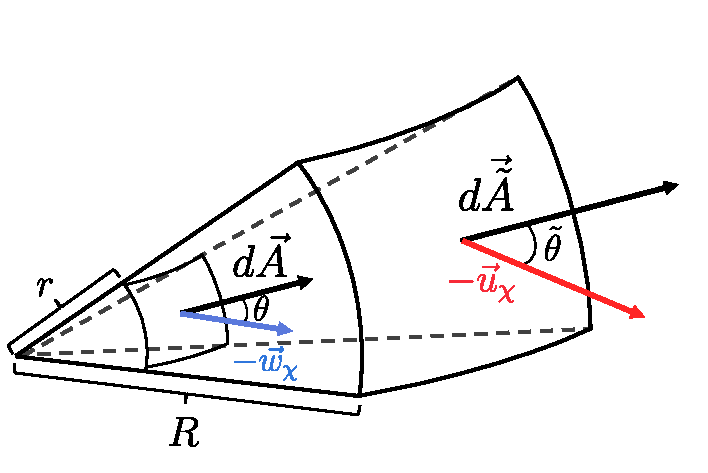
\includegraphics{capture_geometry.pdf}
    \caption{Geometry of the capture process, showing two elements of spheres with radii, $r$ and $R$, near and far from the star respectively.}
    \label{ch3:fig:capturegeometry}
\end{figure}

The probability that the DM interacts with the constituents of the shell depends on the interaction rate, $\Omega(w_\chi)$, multiplied by the time spent in the shell, $dt = dr/\dot r$. Hence, the probability of scattering within the shell is
\begin{equation}
    \Omega(w_\chi) \frac{dr}{\dot r} = 2  \Omega(w_\chi)\frac{1}{w_\chi}\left(1 - \left(\frac{J_\chi}{r w_\chi}\right)^2 \right)^{-1/2} \Theta(J_{\mathrm{max}} - J_\chi)\,dr,\label{ch3:eq:int_prob_1}
\end{equation}
where the factor of 2 is due to the DM having two opportunities to pass through the shell, once when incoming and another after turning around\footnote{The radial velocity $\dot r$ is a standard result in orbital mechanics and can be obtained from the central force Lagrangian.}. The step-function is put in to ensure the angular momentum does not exceed its maximum allowed value. 

For a scattered DM to be considered captured, it must lose enough energy in the collision to become gravitationally bound. The rate at which a DM particle scatters from an initial velocity $w_\chi$ to a final velocity $v<v_e(r)$ is given by~\cite{Gould:1987ju_WeaklyInteractingMassive, Gould:1987ir_ResonantEnhancementsWIMP, Busoni:2017mhe_oct_Evaporationscatteringmomentum}
\begin{align}
    \Omega^{-}(w_\chi) &= \int_0^{v_e} R^-(w_\chi \rightarrow v) dv,\label{ch3:eq:down_rate_1}\\
    R^-(w_\chi \rightarrow v) & = \int n_T(r) \frac{d\sigma_{\chi T}}{dv} |\vec{w}_\chi -\vec{u}_T| f_T(u_T) \,d^3\vec{u}_T, \label{ch3:eq:diff_int_NR_gen}
\end{align}
with $R^-(w_\chi \rightarrow v)$ being the differential interaction rate, $n_T$ is the target number density, $u_T$ is the target velocity and $f_T(u_T)$ is the corresponding distribution function, and $d\sigma_{\chi T}/dv$ is the differential cross-section. The minus superscript is used to signify that this is the down scattering rate, i.e. the rate of interactions leading to the DM losing energy. 

Finally, we obtain the capture rate by multiplying Eqs.~\ref{ch3:eq:shell_flux} and~\ref{ch3:eq:int_prob_1} and integrate over the angular momentum to give the result
\begin{equation}
    C =\int_0^{R_\star} \,dr\, 4\pi r^2 \int_0^\infty\,du_\chi\, \frac{\rho_\chi}{m_\chi} \frac{\fMB(u_\chi, \Tstar)}{u_\chi} w_\chi(r)\Omega^-(w_\chi).
\end{equation}
This result is rather generic, as the choice of DM model will only dictate the form of the differential cross-section in  Eq.~\ref{ch3:eq:diff_int_NR_gen}. As written above, the distribution function for the relative velocity far from the star can be any isotropic distribution function. The MB form was chosen as it allows for a simple analytic form of the total capture rate. 

% To give a simple example, we neglect the thermal motion of the constituents, reducing the rate to
% \begin{align}
%     R^-(w_\chi \rightarrow v) = \frac{4 \mu_+^2}{\mu} n_T \frac{v}{w_\chi} \frac{d\sigma_{\chi T}}{d\cos\theta_{\mathrm{CM}}} \Theta\left(v - w\frac{|\mu_-|}{\mu_+}\right).
% \end{align}
% where $n_T$ is the local number density of the targets, and we have introduced the useful quantities $\mu$, $\mu_\pm$ that are
% \begin{equation}
%     \mu = \frac{m_\chi}{\mi}, \quad  \mu_\pm = \frac{\mu \pm 1}{2}.
% \end{equation}
% For the case of constant DM-target cross-section, we can compute the integral in Eq.~\ref{ch3:eq:down_rate_1}
% \begin{align}
%     R^-(w_\chi \rightarrow v) &= \frac{4 \mu_+^2}{\mu} n_T \frac{v}{w_\chi}\frac{\sigma_{\chi T}}{2} \Theta\left(v - w\frac{|\mu_-|}{\mu_+}\right),\\
%     \Omega^-(w_\chi) & = \frac{2\mu_+^2}{\mu} \frac{n_T \sigma_{\chi T}}{w_\chi} \left(v_e^2 - \frac{\mu_-^2}{\mu_+^2}w_\chi^2\right)\Theta\left(v_e^2 - \frac{\mu_-^2}{\mu_+^2}w_\chi^2\right).
% \end{align}

% It may be the case that the DM does not lose enough energy in a single scatter to become gravitationally bound to the star. If so, the capture probability must be modified for multi-scatter capture. \commMV{Gould and Bramante...}

%%%%%%%%%%%%%%%%%%%%%%%%%%%%%%%%%%%%%
%%%%%%%%%%%%%%%%%%%%%%%%%%%%%%%%%%%%%
%%%%%%%%%%%%%%%%%%%%%%%%%%%%%%%%%%%%%
\section{Capture in Compact Objects}
\label{ch3:sec:captrue_new_full}
%%%%%%%%%%%%%%%%%%%%%%%%%%%%%%%%%%%%%
%%%%%%%%%%%%%%%%%%%%%%%%%%%%%%%%%%%%%
%%%%%%%%%%%%%%%%%%%%%%%%%%%%%%%%%%%%%

Having reviewed the capture process in non-relativistic stars, we can begin discussing the necessary modifications required when considering relativistic stars. In this section, we consider the two major modifications that need to be made: 
\begin{itemize}
    \item The corrections from General Relativity due to the extreme gravitational fields. This ultimately alters the flux of DM passing through the star, boosting it through gravitational focusing.
    \item Accounting for the relativistic and degenerate nature of the star's constituents in the interaction rate.
\end{itemize}

The former is generic to neutron stars and white dwarfs, while the latter is required for all NS constituents, but only the electrons in a WD are degenerate and relativistic. The ions of the WD are non-relativistic and non-degenerate and, hence, can the solar capture formalism can be applied in this case. 

%%%%%%%%%%%%%%%%%%%%%%%%%%%%%%%%%%%%%
%%%%%%%%%%%%%%%%%%%%%%%%%%%%%%%%%%%%%
\subsection{General Relativistic Corrections to the Capture Rate}
\label{ch3:subsec:GR_corr_capture}
%%%%%%%%%%%%%%%%%%%%%%%%%%%%%%%%%%%%%
%%%%%%%%%%%%%%%%%%%%%%%%%%%%%%%%%%%%%

Far from the star, the physics is the same as in the previous section. The deviations arise as the DM falls into he gravitational potential of the star. We begin by following the DM along its trajectory, moving from a distance $R\gg R_\star$ to a closer distance $r$. Hence, we are working in the DM rest frame and calculating the rate at which the DM passes through the shell \textit{per unit of proper time}, $\tau$. The proper time interval is related to the metric through
\begin{equation}
    d\tau^2 = B(r) dt^2 - A(r) dr^2 - r^2 d\Omega^2,
\end{equation}
with $B(r)$ and $A(r)$ defined in Chapter~\ref{chapter:compactobjects}. 

Following the same arguments as in the non-relativistic case, the flux of DM passing through the shell is 
\begin{equation}
    \frac{d N_\chi}{d\tau} = 2\pi \frac{\rho_\chi}{m_\chi}\frac{\fMB(u_\chi)}{u_\chi}\,du_\chi\,\frac{J_\chi \, dJ_\chi}{m_\chi^2},
\end{equation}
which takes the same form as Eq.~\ref{ch3:eq:shell_flux}, with the physical difference being that this is the rate with respect to the proper time. Additionally, as we will be considering cold stars, we take the $\Tstar\rightarrow 0$ limit of the DM-target relative velocity distribution, such that 
\begin{align}
    f_{\mathrm{MB}}(u_\chi) & = \lim_{\Tstar\rightarrow 0}f_{\mathrm{MB}}(u_\chi, \Tstar)\\
    & = \frac{u_\chi}{v_\star} \sqrt{\frac{3 }{2 \pi (v_d^2 + 3 T_\star /\mi)}} \left( e^{-\frac{3(u_\chi - v_\star)^2}{2(v_d^2 + 3 T_\star /\mi)}} - e^{-\frac{3(u_\chi + v_\star)^2}{2(v_d^2 + 3 T_\star /\mi)}} \right),
    \label{ch3:eq:MB}
\end{align}

The probability that DM scatters within the shell and is captured is $2\hat{\Omega}^-(r) d\tau$,
where $\hat{\Omega}^-(r)$ is the interaction rate with respect to the proper time, and $d\tau$ is the proper time taken to move from coordinate $r$ to $r + dr$. The factor of 2 once again accounts for the DM crossing the shell twice per orbit. For calculation purposes, we need to relate this to the interaction rate seen by a distant observer, $\Omega^-(r)$, that is done through
\begin{equation}
    \hat{\Omega}^-(r) d\tau = \frac{1}{\sqrt{g_{tt}}}\Omega^-(r)d\tau= \frac{1}{\sqrt{B(r)}}\Omega^-(r)d\tau.
\end{equation}
Now, the proper time that the DM spends inside a shell of thickness $dr$ will be\footnote{See Appendix~\ref{appendix:kin_heating} for the derivation of $\dot r = \frac{dr}{dt}$.}
\begin{equation}
    d\tau = \left( \frac{d\tau}{dt}\right) dt = B(r) \frac{dr}{\dot r} = \frac{\sqrt{B(r)} dr}{\sqrt{\frac{1}{A(r)} \left[ 1 - B(r)\left( 1 + \frac{J_\chi^2}{m_\chi^2 r^2} \right) \right]}}.
\end{equation}

The differential capture rate can then be written as 
\begin{equation}
    dC =  2\pi  \frac{\rho_\chi}{m_\chi}\frac{\fMB(u_\chi)}{u_\chi}\,du_\chi\,\frac{dJ^2_\chi}{m_\chi^2} \frac{\Omega^-(r)\sqrt{A(r)} \,dr}{\sqrt{1 - B(r)\left( 1 + \frac{J_\chi^2}{m_\chi^2 r^2} \right)}}.
\end{equation}
As the total number of targets in the star, $N_T$, needs to satisfy
\begin{equation}
    N_T = \int_0^{R_\star} 4\pi r^2 n_T(r)\sqrt{A(r)}\,dr,
\end{equation}
where $n_T(r)$ is the number density that appears in the interaction rate, we absorb the factor $\sqrt{A(r)}$ into the definition of $n_T(r)$, such that $\Omega^-(r)\sqrt{A(r)}\rightarrow \Omega^-(r)$. This is due to the number densities obtained by solving the TOV equations already account for the $\sqrt{A(r)}$ factor. 

As before, we have $w_\chi^2(r) = u_\chi^2 + v_e^2(r)$, however as the escape velocity will be significantly larger than the ambient DM velocity far from the star, we can safely approximate $w_\chi^2(r)\approx v_e^2(r)$. 
In the relativistic case, the escape velocity can be defined as
\begin{equation}
    v_e^2(r) = \left(\frac{dl}{d\tau}\right)^2 = A(r) \left(\frac{dr}{d\tau}\right)^2 + r^2 \left(\frac{d\phi}{d\tau}\right)^2 = 1 - B(r),
    \label{ch3:eq:vesceq}
\end{equation}
where $dl$ is a length element. 
The large boost from the escape velocity also removes the $u_\chi$ dependence in the kinematics of the interactions and allows us to perform the integration over the initial DM velocity, yielding an overall factor of
\begin{equation}
    \int_0^\infty \frac{\fMB(u_\chi)}{u_\chi} du_\chi = \frac{1}{v_\star}\erf\left(\sqrt{\frac{3}{2}}\frac{v_\star}{v_d}\right).
\end{equation}

To integrate over $J^2_\chi$, we need the maximum angular momentum the DM can achieve as it passes through the shell. This can be obtained by requiring the argument of the radical above to remain positive, giving
\begin{equation}
    J_\mathrm{max} = \sqrt{\frac{1 - B(r)}{B(r)}} m_\chi r.
\end{equation}
The factor of $1/\sqrt{B}$ arises due to the gravitational focusing of the incoming flux of DM~\cite{Kouvaris:2007ay_WIMPAnnihilationCooling}.
% The angular momentum is given by
% \begin{equation}
%     J_\chi = m_\chi r^2\frac{d\phi}{d\tau}  \leq \frac{m_\chi}{\sqrt{B(r)}} r w_\chi(r) = J_\mathrm{max},
% \end{equation}
% This can be obtained by requiring that the contents of the square root above remain positive, giving
% \begin{equation}
%     J_\mathrm{max}^2 = \frac{1-B(r)}{B(r)} m_\chi^2 r^2,
% \end{equation}

Putting everything together, and integrating over the radius of the star, we are left with the final result for the capture rate of
\begin{equation}
    C =\frac{4\pi}{v_\star}\frac{\rho_\chi}{m_\chi} \erf\left(\sqrt{\frac{3}{2}}\frac{v_\star}{v_d}\right) \int_0^{R_\star}  r^2\frac{\sqrt{1 - B(r)}}{B(r)}\Omega^-(r)\,dr.
    \label{ch3:eq:cap_rel_full_1}
\end{equation}
All that remains is determining the form of the interaction rates for relativistic energies.


%%%%%%%%%%%%%%%%%%%%%%%%%%%%%%%%%%%%%
%%%%%%%%%%%%%%%%%%%%%%%%%%%%%%%%%%%%%
\subsection{Geometric Limit and Threshold Cross-Section}
\label{ch3:subsec:geom_lim_threshold_xs}
%%%%%%%%%%%%%%%%%%%%%%%%%%%%%%%%%%%%%
%%%%%%%%%%%%%%%%%%%%%%%%%%%%%%%%%%%%%

In the previous section, we derived an expression for the capture rate assuming that the DM is captured after a single scatter, and that it only scatters once along its orbit through the NS. This first assumption is true for DM light enough to lose enough energy in this single interaction, which for nucleon targets turns out to be $m_\chi\lesssim 10^6\GeV$. The latter assumption is a statement that we are working in the optically thin regime, such that the cross-section is much less than the ``threshold cross-section'', $\sigmath$. The value of the threshold cross-section is defined as the cross-section for which the capture rate evaluated in the optically thin regime is equal to the geometric limit \cite{Bell:2018pkk_sep_HeatingNeutronStars},  
%
\begin{equation}
C_\mathrm{geom} =  \frac{\pi R_\star^2(1-B(R_\star))}{v_\star B(R_\star)} \frac{\rho_\chi}{m_\chi} \erf\left(\sqrt{\frac{3}{2}}\frac{v_\star}{v_d}\right).
\label{ch3:eq:capturegeom}
\end{equation}
% 
This is the capture rate for which the entire flux of DM passing through the surface of the star is captured at the surface. Hence, it serves as an upper bound to the capture rate, with cross-sections greater than $\sigmath$ saturating the capture rate to this value.
Note the $1/B(\Rstar)$ factor in the equation above. In stars and planets where classical Newtonian mechanics can be applied, gravitational focusing would result in a factor  $v_{esc}^2/\vstar =  (1-B(\Rstar))/\vstar$ in Eq.~\ref{ch3:eq:capturegeom}, where we have used Eqs.~\ref{ch3:eq:vesceq} and \ref{ch2:eq:B_boundary_condition}. 
In neutron stars, on the other hand, general relativity introduces an additional factor of $1/B(\Rstar)$, which can be obtained from the derivation of the flux of DM particles accreted to a NS with a Schwarzschild metric (Eq.~\ref{ch3:eq:cap_rel_full_1})~\cite{Goldman:1989nd_WeaklyInteractingMassive,Kouvaris:2007ay_WIMPAnnihilationCooling}.

For scattering on neutrons, the threshold cross-section is approximately
\begin{align}
\sigma_{th} =  \begin{cases}
\, \sigma_\mathrm{ref} \frac{\GeV}{m_\chi}, \quad &m_\chi \lesssim 1\GeV \quad \ \ \text{ (Pauli blocking  regime)}, \\
\, \sigma_\mathrm{ref}, \quad &1\GeV \lesssim m_\chi \lesssim 10^6\GeV,  \\
\, \sigma_\mathrm{ref} \frac{m_\chi}{10^6\GeV}, \quad &m_\chi\gtrsim 10^6\GeV \quad  \text{(Multiscattering regime)},
\end{cases}
\label{ch3:eq:sigmath}
\end{align}
where we take the canonical value of
\begin{equation}
    \sigma_\mathrm{ref}\sim 1.7 \times 10^{-45}\cm^2,
\end{equation}
which assumes the NS is a solid sphere such that $\sigmaref\sim m_n \pi \Rstar^2/\Mstar$ with $m_n$ the neutron mass.

For scattering off other targets, Pauli blocking is relevant for $\qomax \lesssim  \mu_{\rm target}$ 
while multi-scattering is relevant for $m_\chi \gtrsim \qomax/v_{\star}^2$, where $\qomax$ is the maximum energy transfered in a collision, as will be discussed later.  In addition, because the other target species have a lower abundance than neutrons, the reference cross-section, $\sigma_\mathrm{ref}$, will be higher. The values of $\sigma_{th}$ in Eq.~\ref{ch3:eq:sigmath}, and their regions of applicability, can thus be altered appropriately for other target species of interest.

%%%%%%%%%%%%%%%%%%%%%%%%%%%%%%%%%%%%%
%%%%%%%%%%%%%%%%%%%%%%%%%%%%%%%%%%%%%
\subsection{Interaction Rate for Relativistic Energies and Degenerate Targets}
\label{ch3:subsec:int_rate_degen_rel}
%%%%%%%%%%%%%%%%%%%%%%%%%%%%%%%%%%%%%
%%%%%%%%%%%%%%%%%%%%%%%%%%%%%%%%%%%%%

Our next goal is to write down an interaction rate suitable for describing the interactions between relativistic particles and account for the degeneracy of the target species. This will be achieved by modifying the non-relativistic interaction rate of Eq.~\ref{ch3:eq:down_rate_1} through the use of relativistic kinematics and the use of Lorentz invariant quantities, and the correct distribution functions for degenerate fermion targets.

As shown in Eqs.~\ref{ch3:eq:down_rate_1} and~\ref{ch3:eq:diff_int_NR_gen}, the interaction rate between non-relativistic, non-degenerate species $i$ can be expressed as
\begin{equation}
    \Omega^{-}(r) = \int dv \frac{d\sigma}{dv} |\vec{w}_\chi -\vec{u}_i| n_i(r) \fMB(u_i)d^3u_i.
    \label{ch3:eq:NR_int_rate_simple}
\end{equation}
First, we address the degeneracy of the targets by exchanging the Maxwell-Boltzmann distribution function for a Fermi-Dirac (FD) distribution, $\fFD(\Ei,r)$, via the replacement
\begin{equation}
    n_i(r) \fMB(u_i)d^3 u_i \rightarrow \frac{g_s}{(2\pi)^3}\fFD(\Ei, r),
    \label{ch3:eq:number_density_replacement}
\end{equation}
where $g_s = 2$ is the number of spin states of the target species, $p$ is the 3-momentum of the incoming target, and $\Ei$ is its corresponding energy. The radial dependence of the FD distribution stems from its implicit dependence on the chemical potential of the target. Rewriting this expression in a more computationally friendly manner in terms of the relevant kinematic quantities results in 
\begin{equation}
    \frac{g_s}{(2\pi)^3}\fFD(\Ei, r) = \frac{p \Ei}{2\pi^2}\fFD(\Ei, r) d\Ei d\cos\theta_{uw},
    \label{ch3:eq:free_Fermi_number}
\end{equation}
where we have expressed the angular component of the $d^3 p$ differential in terms of the angle between the incoming DM and target. This angle can be traded for the more useful quantity $s$, the centre of mass energy through
\begin{equation}
    \frac{d\cos\theta_{uw}}{ds} = \frac{1}{2 p p_\chi} = \frac{1}{2 p \sqrt{E_\chi^2 - m_\chi^2}} = \frac{1}{2 p m_\chi}\sqrt{\frac{B(r)}{1 - B(r)}},
\end{equation}
as the initial DM energy is $E_\chi = m_\chi/\sqrt{B(r)}$.

Next, we calculate the initial relative velocity, $|\vec{w}_\chi -\vec{u}_i|$, using relativistic kinematics, expressing it in terms of the Mandalstam $s$, 
\begin{equation}
    |\vec{w}_\chi -\vec{u}_i| = \frac{\sqrt{s^2 - 2 s (1 + \mu^2)\mi^2 + (1 - \mu^2)^2 \mi^4}}{s - (1 + \mu^2) \mi^2},
\end{equation}
where $\mu = m_\chi/\mi$.

Given that it is most common to present the relativistic differential scattering cross-section $d\sigma/d\cos\thetacm$ as a function of the Mandalstam variables $s$ and $t$, with $\thetacm$ the centre of mass frame scattering angle, we make the replacement
\begin{equation}
    dv \frac{d\sigma}{dv} = dt\frac{d\sigma}{dt} = dt \frac{d\sigma}{d\cos\thetacm}\frac{d\cos\thetacm}{t}.
\end{equation}
The final Jacobian factor can be expressed as
\begin{equation}
    \frac{d\cos\thetacm}{dt} = \frac{2s}{s^2 - 2 s (1 + \mu^2)\mi^2 + (1 - \mu^2)^2 \mi^4},
\end{equation}
for the elastic scattering we consider here.

Finally, we note that the first application of this capture formalism was for neutron targets, with the analysis completed before we had considered the additional effects from the form factors and strong interactions discussed in subSection~\ref{ch1:subsec:quark_to_nucleon_EFT}. These effects will be incorporated into this formalism in a self-consistent way next chapter. The initial approach that was taken to account for the fact that we are using realistic neutron number density profiles, despite the expression in Eq.~\ref{ch3:eq:number_density_replacement} being for a free Fermi gas, is to introduce a correction factor as in Ref.~\cite{Garani:2018kkd_may_NewAnalysisNeutron},
\begin{equation}
    \zeta(r) = \frac{n_i(r)}{n_\mathrm{free}(r)},
\end{equation}
where $n_\mathrm{free}(r)$ is obtained by integrating Eq.~\ref{ch3:eq:free_Fermi_number} over all phase space. In the zero-temperature approximation, the result is

\begin{equation}
    n_\mathrm{free}(r) = \frac{1}{3\pi^2}\left[ \kinFi(r)(2\mi + \kinFi(r))\right]^{3/2}.
    \label{ch3:eq:n_free_Fermi}
\end{equation}

Compiling everything together leads to the final expression for the interaction rate being
\begin{equation}
    \begin{split}
        \Omega^-(r) = \int dt\,d\Ei\,ds\,\zeta(r) \frac{d\sigma}{d\cos\thetacm}\frac{\Ei}{2\pi^2 \mi}&\sqrt{\frac{B(r)}{1 - B(r)}} \frac{s}{\beta(s)\gamma(s)}\\
        &\times\fFD(\Ei, r)(1 - \fFD(\Ei', r)),
    \end{split}
    \label{ch3:eq:int_rate_capture_full}
\end{equation}
where we have introduced the helper functions
\begin{align}
    \beta(s) & = s - (\mi^2 + m_\chi^2), \label{ch3:eq:beta_func}\\
    \gamma(s) & = \sqrt{\beta^2(s) - 4 \mi^2 m_\chi^2}.\label{ch3:eq:gamma_func}
\end{align}
We have also introduced the Pauli blocking factor, $1 - \fFD(\Ei', r)$, to account for the phase space available to the final state target. The energy of this final state particle, $\Ei'$, is in general a messy function of $\Ei$, $t$, $s$, and $r$, and can be obtained from the kinematics of the scattering. This result is presented in Appendix~\ref{appendix:kinematics}.

The integration intervals are 
\begin{align}
    t_\mathrm{min} & = - \frac{\gamma(s)}{s},\\
    t_\mathrm{max} & = 0,\\
    s_\mathrm{min} & = \mi^2 + m_\chi^2 + 2 \frac{\Ei \mchi}{\sqrt{B(r)}} - 2\mchi\sqrt{\frac{1 - B(r)}{B(r)}} \sqrt{\Ei^2 - \mi^2}, \\
    s_\mathrm{max} & = \mi^2 + m_\chi^2 + 2 \frac{\Ei \mchi}{\sqrt{B(r)}} + 2\mchi\sqrt{\frac{1 - B(r)}{B(r)}} \sqrt{\Ei^2 - \mi^2}, \\
    E_{i,\mathrm{min}} & = \mi,\\
    E_{i,\mathrm{max}} & = \frac{\mi}{\sqrt{B(r)}}.
\end{align}

As we will be dealing with NSs at low temperatures, we can take the $\Tstar\rightarrow 0$ limit and replace the FD functions with step functions, 
\begin{align}
    \fFD(\Ei, r) &\rightarrow \Theta(\kinFi(r) +\mi - \Ei),\\
    1 - \fFD(\Ei', r) & \rightarrow  \Theta(\Ei'-\mi - \kinFi(r) ).
\end{align}
The first step function can be used to further restrict the $\Ei$ integration interval to be $[\mi, \mi + \kinFi(r)]$. In practice, we work with the kinetic energies of the targets rather than their total energy, as this is the quantity that directly changed in the interactions. Therefore, unless otherwise specified, we will take $\Ei$ to mean the target kinetic energy, with the integration range being $0\le \Ei\le \kinFi$.

This expression resembles that of Ref.~\cite{Garani:2018kkd_may_NewAnalysisNeutron}, but uses a relativistic formalism instead. In Appendix~\ref{app:sec:weakfieldlimit}, we show that Eq.~\ref{ch3:eq:int_rate_capture_full} reduces to the classical expression for the interaction rate in the non-relativistic limit. 


%%%%%%%%%%%%%%%%%%%%%%%%%%%%%%%%%%%%%
%%%%%%%%%%%%%%%%%%%%%%%%%%%%%%%%%%%%%
%%%%%%%%%%%%%%%%%%%%%%%%%%%%%%%%%%%%%
\section{The Differential Interaction Rate}
\label{ch3:sec:diff_int_rate}
%%%%%%%%%%%%%%%%%%%%%%%%%%%%%%%%%%%%%
%%%%%%%%%%%%%%%%%%%%%%%%%%%%%%%%%%%%%
%%%%%%%%%%%%%%%%%%%%%%%%%%%%%%%%%%%%%

In the previous section, we have calculated the interaction rate, $\Omega^-(r)$, assuming the initial DM energy takes its pre-capture value, $E_\chi = \mchi /B(r)$. However, we are also interested in an expression for the interaction rate valid for arbitrary DM energy. This will be required when we consider capture via multiple scatterings, and it will also be necessary to study the subsequent scattering interactions that follow capture and lead to the DM thermalising within the NS.
In principle, it is possible to calculate this rate numerically by binning $\Omega^-$, Eq.~\ref{ch3:eq:int_rate_capture_full}, in the energy loss, i.e. multiplying $\Omega^-$ by $\frac{1}{E_i-E_j}\Theta(E_i+\Ei-\Ei')\Theta(\Ei'-\Ei-E_j)$ and integrating over the bin $[E_j,E_i]$. 
However, it is possible to derive analytic expressions for the differential rate, valid in the zero-temperature approximation. To do so, we use the definition of the scattering rate in Ref.~\cite{Reddy:1997yr_Neutrinointeractionshot,Bertoni:2013bsa_dec_DarkMatterThermalization} 
\begin{equation}
    \begin{split}
        \Gamma^-(E_\chi) &= 2\int \frac{d^3k'}{(2\pi)^3}\int \frac{d^3p}{(2\pi)^3}\int \frac{d^3p'}{(2\pi)^3} \frac{\Msq}{(2E_\chi)(2E'_\chi)(2\Ei)(2\Ei')}\\
        &\hspace{4em}\times(2\pi)^4\delta^4\left(k_\mu+p_\mu-k_\mu'-p_\mu'\right) \fFD(\Ei)(1-\fFD(\Ei')),
    \end{split}
\label{ch3:eq:scattrate}
\end{equation}
where $\Msq$ is the squared matrix element,
$k^\mu=(E_\chi,\vec{k})$ and $k^{'\mu}=(E'_\chi,\vec{k'})$ are the DM initial and final momenta, and $p^\mu=(\Ei,\vec{p})$ and $p^{'\mu}=(\Ei',\vec{p'})$ are the target particle initial and final momenta, respectively.
To see that $\Gamma^-$ is indeed the same as $\Omega^-$ in Eq.~\ref{ch3:eq:int_rate_capture_full}, multiply and divide by
$v_{rel}=|\vec{w}-\vec{u}_i|$ to reintroduce the quantum field theoretic definition of differential cross-section, 
\begin{align}
    d\sigma & = \frac{\Msq}{2 E_\chi 2\Ei|\vec{w} - \vec{u}_i|}d^2\Pi_\mathrm{LIPS},\label{ch3:eq:diffxsec}\\
    d^2\Pi_\mathrm{LIPS} &= \frac{1}{2E'_\chi}\frac{d^3 k'}{(2\pi)^3}\frac{1}{ 2\Ei'}\frac{d^3 p'}{(2\pi)^3}(2\pi)^4\delta^4(k_\mu + p_\mu - k'_\mu - p'_\mu),\\
    \implies\frac{d\sigma}{d\cos\thetacm} &= \frac{1}{16 \pi}\frac{\beta(s)}{2 s \beta(s) - \gamma^2(s)}\Msq,
\end{align}
where $d^2\Pi_\mathrm{LIPS}$ is the 2-body Lorentz invariant phase space.

The advantage of Eq.~\ref{ch3:eq:int_rate_capture_full} is that it can be used to calculate the capture rate for any interaction given the differential cross-section. The disadvantage is that this computation has to be evaluated numerically, which can be computationally intensive. For this reason, shall now use Eq.~\ref{ch3:eq:scattrate} to derive analytic expressions that will allow us to speed up computations and, in addition, calculate the shape of the interaction rate as a function of the energy loss. 

The interaction rate for $d\sigma \propto s^m t^n$ is 
\begin{equation}
    \begin{split}
        \Gamma^{-}(E_\chi) & \propto \sum_{n,m}  \frac{(-1)^n }{128\pi^3 E_\chi k }\int_0^{E_\chi -m_\chi} dq_0\int \frac{dt_E t_E^n}{(t_E + q_0^2)^{m+\frac{1}{2}}}\\
        &\hspace{4em}\times\sum_{r=0}^m \mathcal{V}_{m,r}\sum_{j = 0}^r\binom{r}{j} \kinFi^{r-j}  \frac{(-1)^{j} q_0^{j+1}}{j+1} h_j\left( \frac{\Ei^{t^-} - \kinFi}{q_0}\right),
    \end{split}
    \label{ch3:eq:gamma_full_text}
\end{equation}
for elastic scattering with $t_E=-t=q^2-q_0^2$, where $q_0=\Ei'-\Ei$ is the DM energy loss, 
\begin{equation}
\Ei^{\, t^{-}} = -\left(m_n+\frac{q_0}{2}\right) + \sqrt{\left(m_n+\frac{q_0}{2}\right)^2+\left(\frac{\sqrt{q^2-q_0^2}}{2}-\frac{m_n q_0}{\sqrt{q^2-q_0^2}}\right)^2}, 
\label{ch3:eq:Etm_def}
\end{equation}
is the minimum energy of the neutron before the collision, obtained from kinematics,  and $h_j(x)$ is a step function with a smooth transition, 
\begin{equation}
    h_j(x) = \begin{cases}
        & 0, \quad x >0\\
        & (-x)^{j+1},\quad -1<x <0\\
        & 1,\quad x<-1
    \end{cases}.
    \label{ch3:eq:h_stepfn}
\end{equation}
The full derivation of this interaction rate can be found in Appendix~\ref{appendix:interaction_rates}. 
Our result for $\Gamma^-$ is an extension of that presented in Ref.~\cite{Bertoni:2013bsa_dec_DarkMatterThermalization}, where the interaction rate was calculated only in the case of low energy and a constant matrix element. It is valid at all energy ranges.
The differential interaction rate $\frac{d\Gamma}{d q_0}(E_\chi,q_0)$ is then just the integrand of Eq.~\ref{ch3:eq:gamma_full_text}.
We will use $\frac{d\Gamma}{d q_0}$ to obtain normalised shapes for the differential interaction spectrum, while we will use $\Omega^-$ when we need the total interaction rate, such as in the capture rate. 


%%%%%%%%%%%%%%%%%%%%%%%%%%%%%%%%%%%%%%%
\begin{figure}[t!bp]
    \centering
    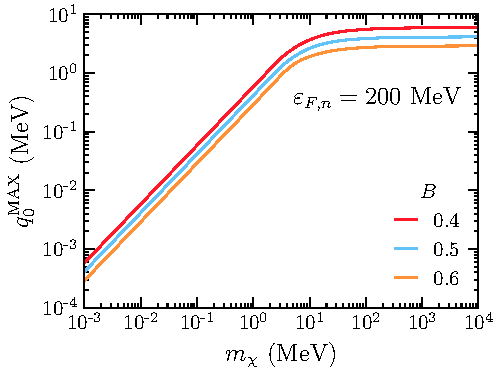
\includegraphics[width = 0.495\textwidth]{capture_1/q0max_mdm.pdf}
    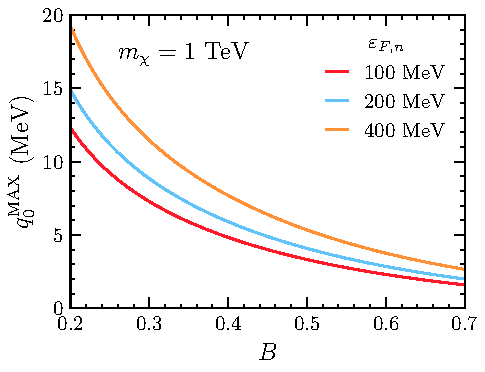
\includegraphics[width = 0.495\textwidth]{capture_1/q0max_B.pdf}

    \caption{Left: $\qomax$ vs. $m_\chi$ for $\kinFn=200\MeV$ and different values of B. 
    Right: $\qomax$ as a function of $B$ for different values of $\kinFi$ and $m_\chi=1\TeV$.}
    \label{ch3:fig:q0max}
\end{figure}
%%%%%%%%%%%%%%%%%%%%%%%%%%%%%%%%%%%%%%

%%%%%%%%%%%%%%%%%%%%%%%%%%%%%%%%%%%%%%
\begin{figure}[t!bp]
    \centering
    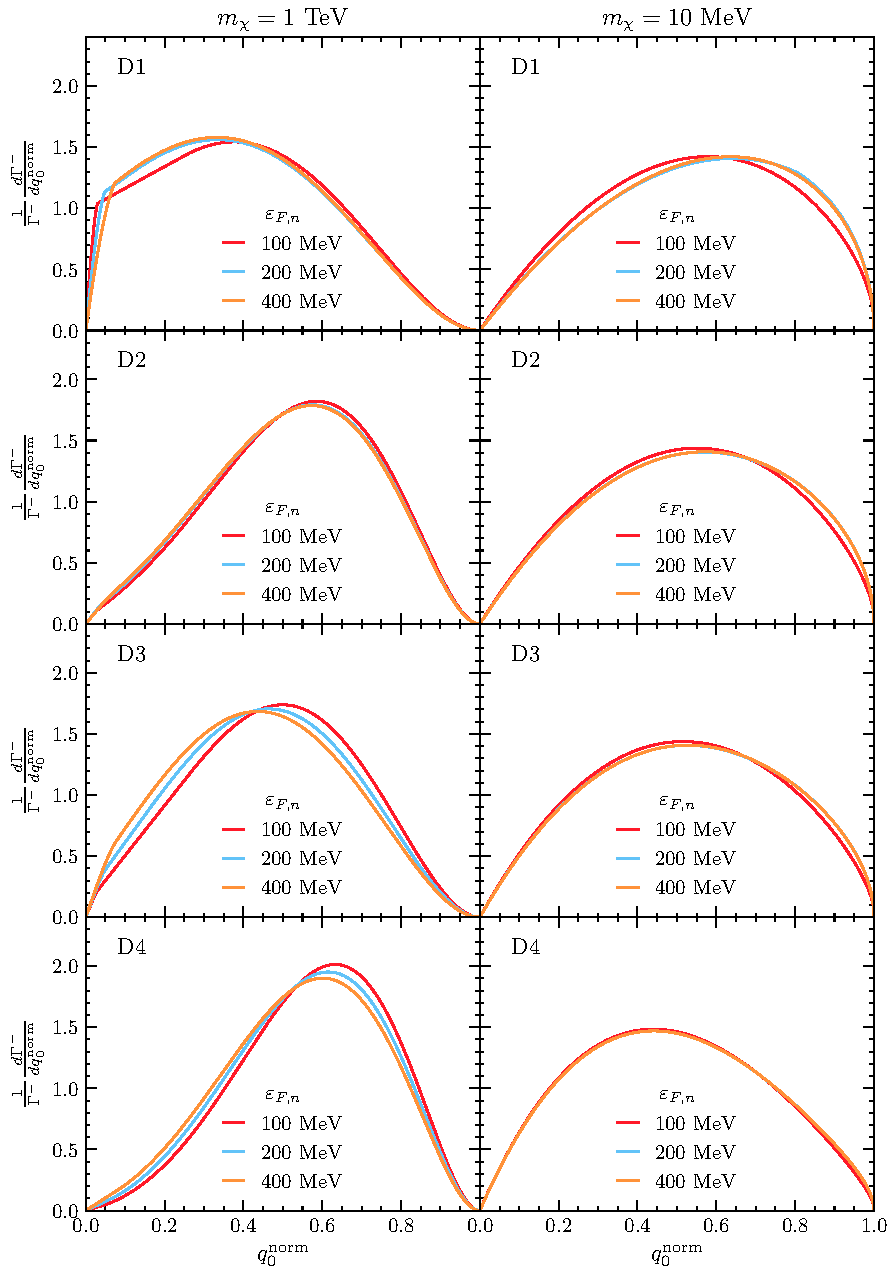
\includegraphics[width = 0.87\textwidth]{capture_1/norm_diff_intrate.pdf}    
    \caption[Normalised differential interaction rates $\frac{1}{\Gamma}\frac{d\Gamma}{d\qonorm}$ as a function of $\qonorm$.]{Normalised differential interaction rates $\frac{1}{\Gamma}\frac{d\Gamma}{d\qonorm}$ as a function of $\qonorm$ for different values of $\kinFn$, $m_\chi=1\TeV$ (left) and $m_\chi=10\MeV$ (right), $B=0.5$ and  operators D1 (first row), D2 (second row), D3 (third row) and D4 (fourth row). Profiles do not depend on $m_\chi$ in the limits $m_\chi\gg m_n$ (left) and $m_\chi\ll m_n$ (right).  }
    \label{ch3:fig:diffintratesd14}
\end{figure}
%%%%%%%%%%%%%%%%%%%%%%%%%%%%%%%%%%%%%%


Kinematics, and the phase space allowed by $h_j(x)$ in Eq.~\ref{ch3:eq:gamma_full_text}, determine the maximum energy that a DM particle can lose in a single scattering interaction, $\qomax$. The details of how to obtain $\qomax$ are given in Appendix~\ref{app:subsec:down_scatter_derivation}.
For DM capture, the value of $\qomax$ depends primarily on the DM mass, as is illustrated in the left panel of Fig.~\ref{ch3:fig:q0max}. We can see that for low $m_\chi$, $\qomax\propto m_\chi$, while, for $m_\chi\gg m_n$, it plataues to values between $\qomax\sim 3 - 6 \GeV$. 
%
Both $\qomax$ and $\frac{d\Gamma}{dq_0}$ also depend on $\kinFn$ and $B$. Changing $\kinFn$ has a very mild effect on the value of $\qomax$ (see right panel of Fig.~\ref{ch3:fig:q0max}) and on the shape of the normalised spectrum (see Fig.~\ref{ch3:fig:diffintratesd14}). On the other hand, increasing $B$ has the main effect of reducing   $\qomax$ (see right panel of Fig.~\ref{ch3:fig:q0max}), but only a mild effect on the shape of the profile expressed as a function of the normalised energy loss 
\begin{equation}
    \qonorm = \frac{q_0}{\qomax}. 
\end{equation}

We apply our results for $\frac{d\Gamma}{d q_0}$ to DM-neutron interactions, and in particular those with differential cross-sections that depend only on the transferred momentum $t=(k^\mu-k^{'\mu})^2$ and not on the centre of mass energy $s=(p^\mu+k^\mu)^2$.

In Fig.~\ref{ch3:fig:diffintratesd14} we show the normalised differential rates as a function of $\qonorm$ for the four operators D1-D4. The left-hand panels are in the limit $m_\chi\gg m_n$. We can observe that D1 has a softer spectrum, while the D2 and D4 spectra peak towards higher values of $q_0$. Varying the chemical potential $\kinFn$ has a very mild effect, shifting the spectrum to lower values of $q_0$ with increasing values of $\kinFn$.
Note that at small values of $\qonorm$ there is a sudden change in the slope of the normalised differential rate, which occurs for all operators but is more evident in D1 (top left panel). This is due to the zero temperature approximation, implicit in Eq.~\ref{ch3:eq:gamma_full_text}, where Heaviside functions were used to approximate FD distributions (see Appendix~\ref{app:subsec:down_scatter_derivation}); using a finite temperature would produce a smoother spectrum at small $\qonorm$. 

In the right-hand panels of Fig.~\ref{ch3:fig:diffintratesd14}, we explore the low DM mass region $m_\chi\ll m_n$. 
In this case, all operators give rise to similar profiles, the sole difference being that the peak of the profile is now shifted to lower  $\qonorm$ for D4 in contrast to D1, with intermediate values for D2 and D3. This is a consequence of Pauli blocking, with this effect depending on the specific power of $t$ that dominates the spectrum. Profiles with lower $n$ ($d\sigma\propto t^n$) peak at higher $\qonorm$ (see Fig.~\ref{ch3:fig:diffintratesd14}, right panels). For D4 we have $\Msq\propto t^2$, while the matrix elements of D2 and D3 are linear combinations of $t$ and $t^2$, and D1 is a combination of all powers of $t$. Comparing the right panels of Fig.~\ref{ch3:fig:diffintratesd14} with Fig.~\ref{app:fig:diffgamma}, we observe that the lowest power of $t$ determines the shape of the final differential interaction rate. Finally, varying $\kinFn$ has a very mild effect, this time shifting the spectrum mostly to higher values of $q_0$ for higher $\kinFn$.

The fact that the lowest power of $t$ dictates the features of the differential interaction rate is true also for the interactions that have a dependence on $s$. As such, by understanding the properties of the interaction rates with $\Msq\propto t^n$, we can understand the rates for all the operators in Table~\ref{ch1:tab:opers_defn_full}.


%%%%%%%%%%%%%%%%%%%%%%%%%%%%%%%%%%%%%%%%%
\subsection{Pauli Blocking}
\label{ch3:subsec:PB_cap}
%%%%%%%%%%%%%%%%%%%%%%%%%%%%%%%%%%%%%%%%%
% The DM interaction rate, Eq.~\ref{ch3:eq:scattrate}, is proportional to the number of target particles (nucleons/leptons) in the initial state with energy $\Ei$, and to the number of available final states with energy $\Ei+q_0$. 

The DM interaction rate, Eq.~\ref{ch3:eq:scattrate}, will be proportional to the number of target particles available to scatter off. Classically, this is the total number of targets within the star. However, the quantum degeneracy of the species within compact objects, due to the extreme densities, leads to a reduction in the number of available initial state target particles the DM can scatter off.
To understand this, consider the $T\rightarrow 0$ approximation, in which all initial states with energies $\Ei < \kinFi$ are occupied. These states are known as the ``Fermi sea". In order for the DM to scatter off one of these states, it must impart enough energy to kick the target out of the Fermi sea, such that 
\begin{equation}
    \Ei' = \Ei + q_0 > \kinFi,
\end{equation}
imposing a lower limit on the energy transfer required for an interaction to take place. This effectively reduces the number of available targets to only those with kinetic energies between $\kinFn - q_0$ and $\kinFi$. 
This suppression of the initial state phase space is known as Pauli blocking (PB), and is a completely quantum phenomenon.
In this limit, we necessarily have $\Gamma^-\rightarrow 0$ for $q_0\rightarrow 0$. 
It is also worth noting that Pauli blocking only affects the interaction rate when $q_0\le \kinFn$.


%%%%%%%%%%%%%%%%%%%%%%%%%%%%%%%%%%%%%%%%%
\begin{figure}[t!bp]
    \centering
    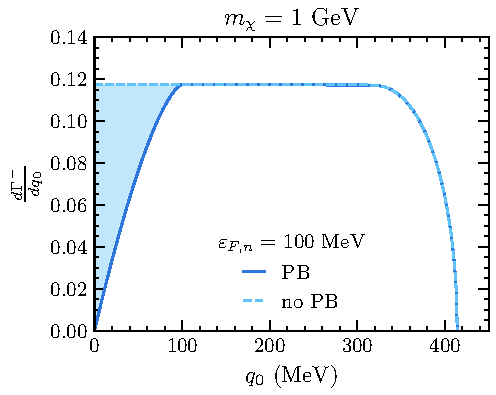
\includegraphics[width=.48\textwidth]{capture_1/diff_intrate_n0_mu_100MeV_mdm1GeV.pdf}
    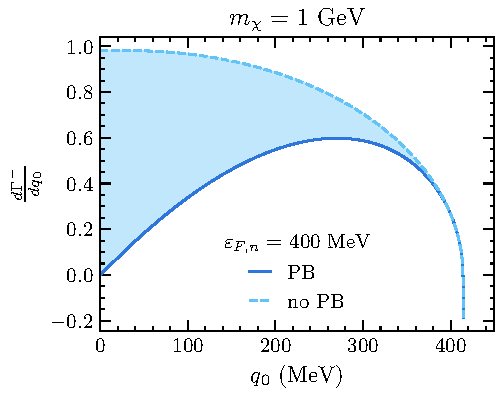
\includegraphics[width=.48\textwidth]{capture_1/diff_intrate_n0_mu_400MeV_mdm1GeV.pdf}\\
    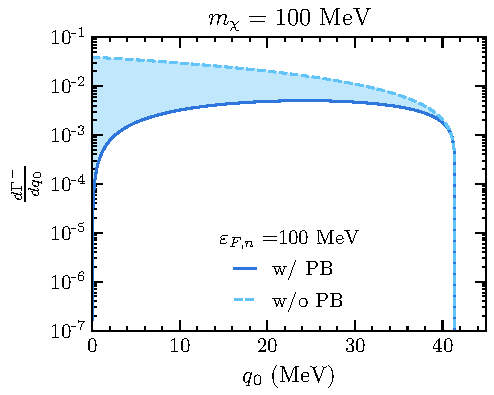
\includegraphics[width=.48\textwidth]{capture_1/diff_intrate_n0_mu_100MeV_mdm100MeV.pdf}
    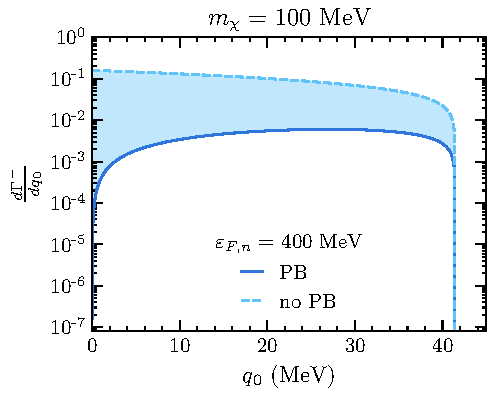
\includegraphics[width=.48\textwidth]{capture_1/diff_intrate_n0_mu_400MeV_mdm100MeV.pdf}\\
    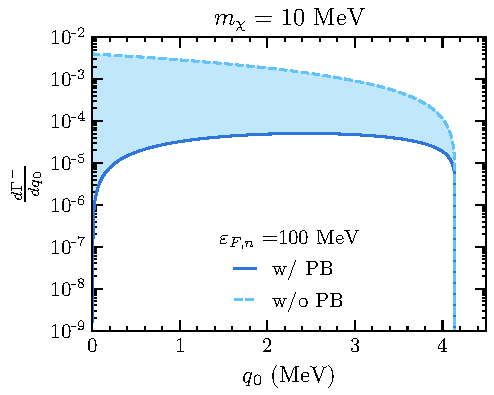
\includegraphics[width=.48\textwidth]{capture_1/diff_intrate_n0_mu_100MeV_mdm10MeV.pdf}
    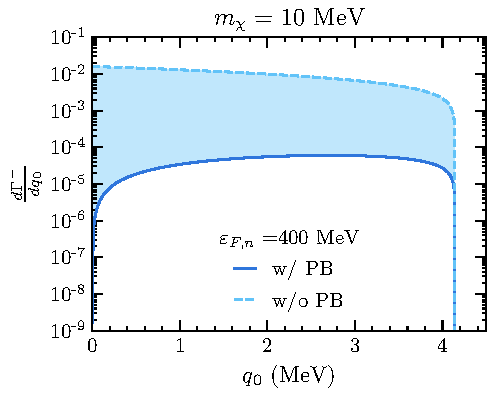
\includegraphics[width=.48\textwidth]{capture_1/diff_intrate_n0_mu_400MeV_mdm10MeV.pdf}
    \caption[Differential interaction rates $\frac{d\Gamma}{dq_0}$  
    as a function of the energy loss $q_0$ for different values of $m_\chi$ and $\kinFn$, constant cross-section and $B=0.5$.]{Differential interaction rates $\frac{d\Gamma}{dq_0}$  
    as a function of the energy loss $q_0$ for different values of $m_\chi$ and $\kinFn$, constant cross-section and $B=0.5$. Blue lines refer to the result that includes Pauli blocking, while the light blue dashed lines refer to the result without PB. Left column:  $\kinFn=100\MeV$, right column: $\kinFn=400\MeV$. Top: $m_\chi=1\GeV$, middle: $m_\chi=100\MeV$, bottom: $m_\chi=10\MeV$.}
    \label{ch3:fig:gammaNPBmu}
\end{figure}
%%%%%%%%%%%%%%%%%%%%%%%%%%%%%%%%%%%%%%%%%




To assess the impact of PB on the DM differential interaction rate, in Fig.~\ref{ch3:fig:gammaNPBmu} we compare the rate 
with (blue solid lines) and without (light blue dashed lines) Pauli blocking, for $B=0.5$ and constant DM-neutron cross-section. When Pauli blocking can be neglected, the interaction rate is obtained straightforwardly from Eq.~\ref{ch3:eq:scattrate} by stripping away the $(1 - \fFD(\Ei'))$ factor. 
The difference between the computations is shaded in light blue. In the top left panel, we see that the rate begins to be suppressed from PB at $q_0 \sim \kinFi = 100\MeV$ for a 1~GeV DM.
% we can see how the differential rate changes by switching Pauli blocking on or off, for $\kinFn=100\MeV$.
%  The rate calculated without PB is flat for $q_0\lesssim 200\MeV$, while when Pauli suppression is active it undergoes a smooth transition towards $0$ for $q_0<\kinFn$. 
In the top right plot, we increase the neutron chemical potential from $\kinFn=100\MeV$ to $\kinFn=400\MeV$. Given that in this case $\qomax \sim 0.4 m_\chi \sim 400\MeV$, almost the whole energy range is affected by PB. The higher $\kinFn$ changes the spectra (both with and without PB) such that the unsuppressed rate is no longer flat at low $q_0$. The PB suppressed rate reaches a maximum at values of $q_0$ slightly below $\qomax$, and then decreases towards $0$ at lower $q_0$.
In the middle panels, $m_\chi=100\MeV$, and $\qomax\sim40\MeV\ll\kinFn$. In this case, it is evident that PB affects the spectrum over the full $q_0=\qomax$ range. In the bottom row, we set $m_\chi=10\MeV$. As expected, for lighter DM,  the effects of PB are even more pronounced.



To understand how the effect of PB varies throughout the star, we can analyse the radial profiles of the capture rates $dC/dr$.
In Fig.~\ref{ch3:fig:diffcap} we plot the differential capture rate as a function of the NS radius, with and without Pauli blocking. We see that Pauli blocking is most significant at low DM mass, below about 1~GeV, and becomes insignificant for higher masses. Pauli blocking has a larger impact on the differential capture rate deeper into the NS interior and has a negligible effect at the surface. This is particularly apparent in the top left panel of Fig.~\ref{ch3:fig:diffcap}. This is because the chemical potential is higher in the NS interior than it is near the crust, as seen in the radial $\kinFi$ profile in the bottom left panel of Fig.~\ref{ch2:fig:BSk_profiles}.

%%%%%%%%%%%%%%%%%%%%%%%%%%%%%%%%%%%%%%%%%
\begin{figure}
    \centering
    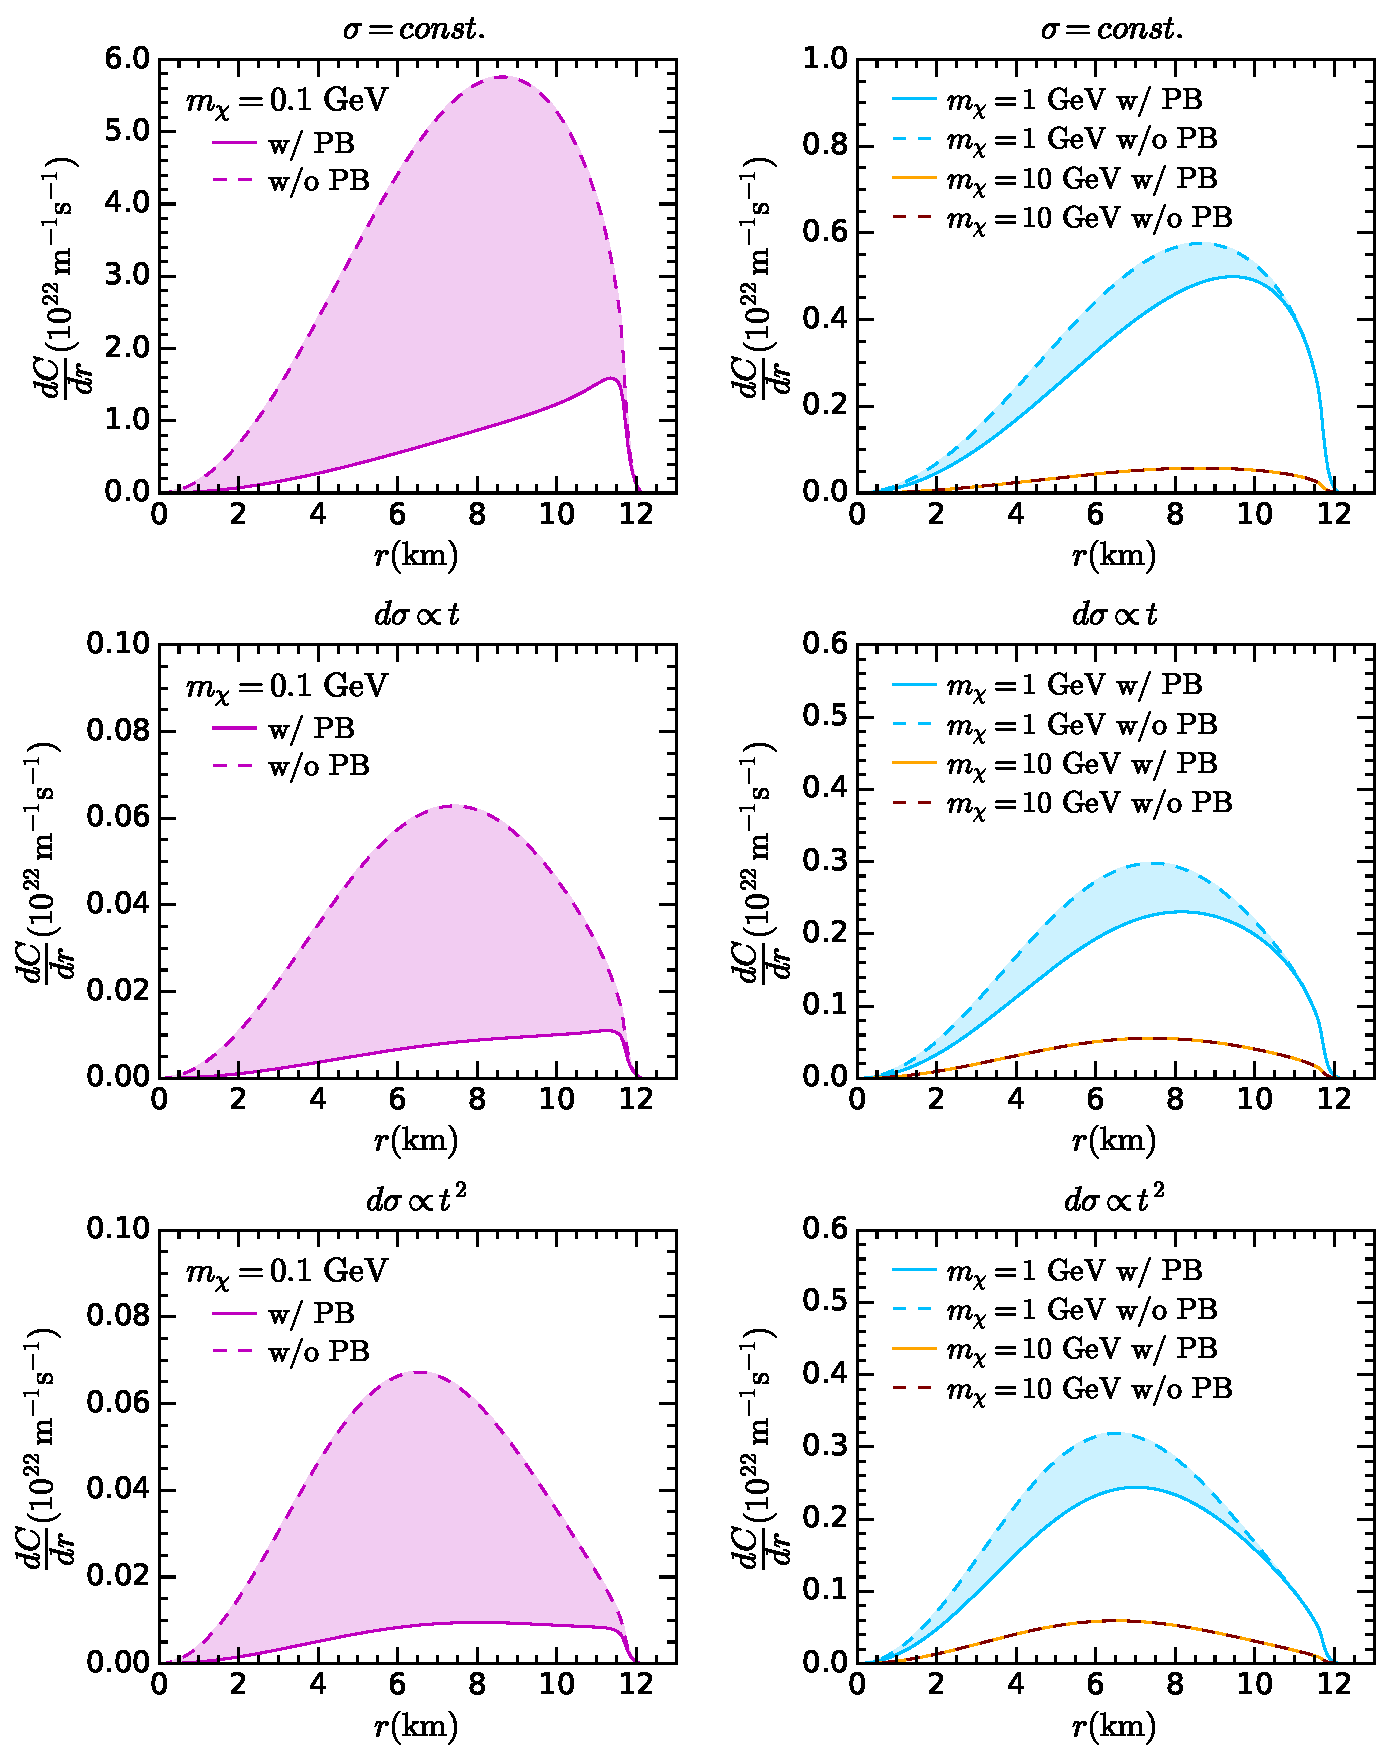
\includegraphics[width=.85\textwidth]{capture_1/diff_cap_rate.pdf}        
    \caption{Differential capture rate as a function of the NS radius $r$, with (solid) and without (dashed) Pauli blocking, for the EoS benchmark BSk24-2. Top: constant cross-section, center: $d\sigma\propto t$, bottom: $d\sigma\propto t^2$.}
    \label{ch3:fig:diffcap}
\end{figure}
%%%%%%%%%%%%%%%%%%%%%%%%%%%%%%%%%%%%%%%%%

%%%%%%%%%%%%%%%%%%%%%%%%%%%%%%%%%%%%%%%%%
%%%%%%%%%%%%%%%%%%%%%%%%%%%%%%%%%%%%%%%%%
%%%%%%%%%%%%%%%%%%%%%%%%%%%%%%%%%%%%%%%%%
\section{Capture in the Low, Intermediate and High Mass Regimes}
\label{ch3:sec:capture_analysis}
%%%%%%%%%%%%%%%%%%%%%%%%%%%%%%%%%%%%%%%%%
%%%%%%%%%%%%%%%%%%%%%%%%%%%%%%%%%%%%%%%%%
%%%%%%%%%%%%%%%%%%%%%%%%%%%%%%%%%%%%%%%%%

Having assembled all the required machinery, we are ready to explore the properties of the capture rate in the three mass regimes outlined in Eq.~\ref{ch3:eq:sigmath}.  Given the computational load required to evaluate Eq.~\ref{ch3:eq:cap_rel_full_1} in general, we aim to provide approximations that are numerically more efficient where possible. We also discuss the high DM mass regime where multiple scatterings are required for capture, and how this is affected by Pauli blocking. 


%%%%%%%%%%%%%%%%%%%%%%%%%%%%%%%%%%%%%%%%%
%%%%%%%%%%%%%%%%%%%%%%%%%%%%%%%%%%%%%%%%%
\subsection{Low and intermediate DM mass range}
\label{ch3:subsec:captureintermediate}
%%%%%%%%%%%%%%%%%%%%%%%%%%%%%%%%%%%%%%%%%
%%%%%%%%%%%%%%%%%%%%%%%%%%%%%%%%%%%%%%%%%


In sections~\ref{ch3:sec:captrue_new_full} and \ref{ch3:sec:diff_int_rate}, we have derived general expressions to numerically calculate the DM capture and interaction rates,  
Eqs.~\ref{ch3:eq:cap_rel_full_1} and \ref{ch3:eq:int_rate_capture_full} respectively.   
Using these expressions, we can write 
the complete expression for the capture rate as a function of the differential DM-neutron cross-section 
\begin{equation}
    \begin{split}
        C = \frac{2\rho_\chi}{\pi \vstar m_\chi^2} {\rm Erf}\left(\sqrt{\frac{3}{2}}\frac{\vstar}{v_d}\right)\int_0^{\Rstar}  dr  \frac{r^2\zeta(r)}{\sqrt{B(r)}} &\int dt d\Ei ds \frac{d\sigma}{d\cos\thetacm}\frac{\Ei s}{\beta(s)\gamma(s)}\\
        &\times \fFD(\Ei,r)(1-\fFD(\Ei',r)), 
    \end{split}
\label{ch3:eq:capturefinal}
\end{equation}
where the functions $\beta$ and $\gamma$ were given in Section~\ref{ch3:subsec:int_rate_degen_rel}. Recall that in the limit $T\rightarrow0$,  $\fFD(\Ei,r)$ and $1-\fFD(\Ei',r)$  reduce to the step functions,  $\Theta(\kinFi(r)-\Ei)$ and  $\Theta(\Ei'-\kinFi(r))$, respectively. 


Exchanging the differential cross-section for the squared matrix allows for easier examination of the operators in Table~\ref{ch1:tab:opers_defn_full}, and so we write the capture rate as
\begin{equation}
    \begin{split}
        C &=  \frac{\rho_\chi}{8\pi^2 \vstar m_\chi^2} {\rm Erf}\left(\sqrt{\frac{3}{2}}\frac{\vstar}{v_d}\right)\int_0^{\Rstar}   dr  \frac{r^2 \zeta(r) }{\sqrt{B(r)}} & \int dt d\Ei ds \frac{\Msq \Ei}{2s\beta(s)-\gamma^2(s)} \frac{s}{\gamma(s)} \\
        &\times \fFD(\Ei,r)(1-\fFD(\Ei',r)). 
    \end{split}
    \label{ch3:eq:capturefinalM2}
\end{equation}
This expression can be used to numerically calculate the single scatter capture rate of DM in compact objects, in the optically thin regime. In general, this must be used for low-mass DM where PB is in effect.

As discussed in Section~\ref{ch3:subsec:PB_cap}, PB eventually becomes negligible for DM with masses $\gtrsim \muFi$. Hence, between this mass and the point where multiple scattering becomes important, PB can be neglected and a simplified capture rate be obtained. For nucleon targets, this range is between $1\GeV\lesssim m_\chi\lesssim 10^6\GeV$, which we call the intermediate mass range.

The resulting simplified capture rate differs slightly depending on whether the matrix element depends only on $t$, or if it has explicit $s$ dependence. We present the full derivations of these results in Appendix~\refeq{app:sec:capratesimple}
First, for $\Msq=a t^n$, the previous expression can be simplified to 
\begin{gather}
        C \sim C_\mathrm{approx} = \frac{4\pi}{\vstar} \frac{\rho_\chi}{m_\chi}{\rm Erf}\left(\sqrt{\frac{3}{2}}\frac{\vstar}{v_d}\right)\int_0^{\Rstar}  r^2 dr \, n_i(r)  \frac{1-B(r)}{B(r)} \langle\sigma(r)\rangle 
\label{ch3:eq:csimplelargemtext}, \\
\langle\sigma(r)\rangle = \left\langle\int dt \frac{d\sigma}{dt} \right\rangle_s =   \frac{a}{16\pi m_\chi^2 } \frac{1}{n+1}\left(\frac{4(1-B(r))m_\chi^2}{B(r)(1+\mu^2)}\right)^{n}. 
\label{ch3:eq:xsecave}
\end{gather}
For $s$-dependent matrix elements the result is very similar, with the only difference being that the cross-section is not averaged over $s$, and instead $s$ is fixed to a particular value as detailed in Appendix~\refeq{app:sec:capratesimple}. Writing the matrix element as $\Msq \propto \bar{g}(s)t^n$, for with $g$ some function of $s$, we arrive at the result
\begin{gather}
    C \sim C_{\mathrm{approx}, s} = \frac{4\pi}{\vstar} \frac{\rho_\chi}{m_\chi}{\rm Erf}\left(\sqrt{\frac{3}{2}}\frac{\vstar}{v_d}\right)\int_0^{\Rstar}  r^2 dr \, n_i(r)  \frac{1-B(r)}{B(r)} \sigma(r)
\label{ch3:eq:csimplelargemtext_sdep}, \\
\begin{split}
    \sigma(r) = \int dt \frac{d\sigma}{dt} & =   \frac{1}{16\pi \left(\mi^2 \mchi^2 + 2\mi \mchi/\sqrt{B(r)}\right)}\frac{\bar{g}(s_0)}{(n+1)}\\
    &\hspace{6em}\times\left[\frac{4(1 - B(r)) \mchi^2}{B(r)(1 + \mu^2) + 2\sqrt{B(r)}\mu}\right]^n,
\label{ch3:eq:xsecave_sdep}
\end{split}\\
s_0 = \mi^2 + \mchi^2 + 2\frac{\Ei\mchi}{\sqrt{B(r)}}.\label{ch3:eq:s0}
\end{gather}
As with the differential interaction rates, it is the $t$-dependence of the matrix elements that dictate the key features of the capture rate.

%%%%%%%%%%%%%%%%%%%%%%%%%%%%%%%%%%%%%%%
\begin{figure}
    \centering
    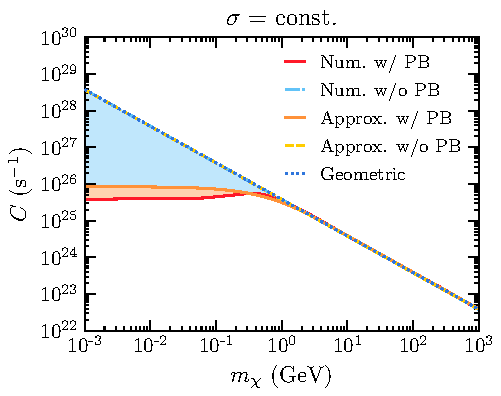
\includegraphics[width=.48\textwidth]{capture_1/capture_rate_n0.pdf}
    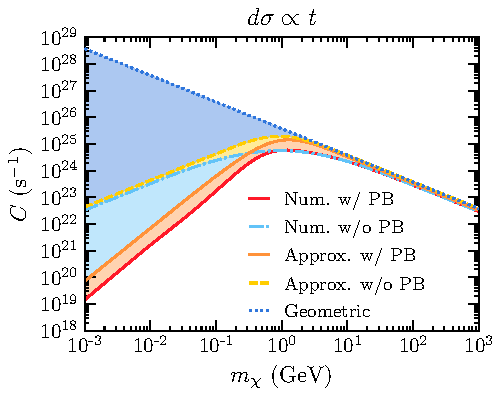
\includegraphics[width=.48\textwidth]{capture_1/capture_rate_n1.pdf}\\
    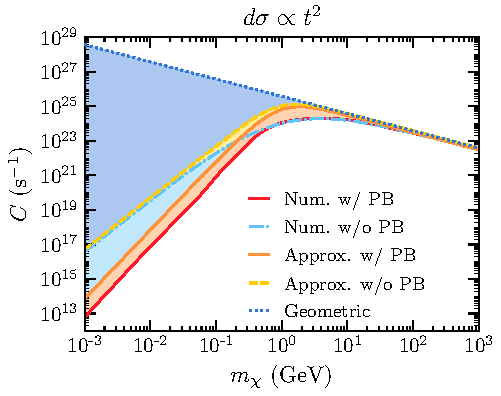
\includegraphics[width=.48\textwidth]{capture_1/capture_rate_n2.pdf}
    \caption[Capture rate as a function of the DM mass with cross-sections normalised to $\sigma=\sigmaref\sim 1.7 \times 10^{-45} \cm^2$, for EoS BSk24-2, calculated with and without Pauli blocking.]{Capture rate as a function of the DM mass with cross-sections normalised to $\sigma=\sigmaref\sim 1.7 \times 10^{-45} \cm^2$, for EoS BSk24-2, calculated with and without Pauli blocking. Top left: constant cross-section. Top right: $d\sigma\propto t$, bottom: $d\sigma\propto t^2$, where $t$ is the Mandelstam variable. All rates are normalised to the geometric limit at large DM mass. }
    \label{ch3:fig:approxc}
\end{figure}
%%%%%%%%%%%%%%%%%%%%%%%%%%%%%%%%%%%%%%%


In Fig.~\ref{ch3:fig:approxc}, we show the capture rate as a function of the DM mass for matrix elements proportional to $t^n$, for $n=0,1,2$ and the NS benchmark model BSk24-2. Numerical results obtained using Eq.~\ref{ch3:eq:capturefinalM2} are shown in solid red; results using the same equation but removing the theta function that enforces Pauli blocking are depicted in light blue; and the approximation for intermediate DM masses, Eq.~\ref{ch3:eq:csimplelargemtext}, in yellow. We show the geometric limit, Eq.~\ref{ch3:eq:capturegeom}, in blue for comparison. 
The capture rates were all normalised to the geometric limit at large DM mass where PB is negligible. 
In the same plots, we also show in brown the result obtained from using a modified version of Eq.~\ref{ch3:eq:csimplelargemtext} to include Pauli blocking.
This is achieved by including the ratio between the differential the interaction rate, $\Gamma^-$, calculated with and without Pauli blocking. This comparison was done in Section~\ref{ch3:subsec:PB_cap} for various values of $B$ and $\kinFn$.

From Fig.~\ref{ch3:fig:approxc}, we can see that Eq.~\ref{ch3:eq:csimplelargemtext} is indeed a good approximation to the numerical results obtained without Pauli blocking, and can be safely used for DM masses from a few $\GeV$ up to $m_\chi\sim10^6\GeV$, where multiple scattering becomes relevant. 
On the other hand, for $m_\chi\lesssim 100\MeV$ the brown line is no longer a good approximation to the numerical result with Pauli blocking, as it always overestimates the capture rate by nearly an order of magnitude. Therefore, to accurately account for the effects of PB for low mass DM, the complete expression for the capture rate, Eq.~\ref{ch3:eq:capturefinalM2} must be used and evaluated numerically.

We now compare our full numerical capture rate calculation, Eq.~\ref{ch3:eq:capturefinalM2}, with that of Ref.~\cite{Garani:2018kkd_may_NewAnalysisNeutron}, in Fig.~\ref{ch3:fig:Cratecomp}. The capture rates calculated in Ref.~\cite{Garani:2018kkd_may_NewAnalysisNeutron} correctly include the stellar structure and Pauli blocking, however, they do not account for general relativistic corrections, and the authors only considered the case of a constant cross-section, $\sigma=10^{-45}\cm^2$. Top make the comparison as fair as possible, we have selected NS configurations that match those of Figs.~1 and 14 of Ref.~\cite{Garani:2018kkd_may_NewAnalysisNeutron}, namely their Model A (BSk20-1):  $\Mstar\simeq1.52\Msun$, $\Rstar\simeq11.6\km$ and Model D (BSk21-2): $\Mstar\simeq2.11\Msun$ and $\Rstar\simeq12.0\km$. We denote these new benchmark models as BSk26-1 (left panel of Fig.~\ref{ch3:fig:Cratecomp}) and BSk24-5 (right panel). Note that we were not able to use the BSk20 and BSk21 functionals, since there are no publicly available fits for the chemical potentials and particle abundances for those EoS families. However, as discussed earlier in section \ref{ch2:subsec:NS_EoS}, BSk26 (BSk24) yields configurations that are almost indistinguishable from those obtained with BSk20 (BSk21)~\cite{Perot:2019gwl_Rolesymmetryenergy}.

We can see in the left panel of Fig.~\ref{ch3:fig:Cratecomp} that in the non-Pauli suppressed region, $m_\chi \gtrsim 1\GeV$, our capture rate calculation in the optical thin limit (solid magenta) exceeds that of Ref.~\cite{Garani:2018kkd_may_NewAnalysisNeutron} (dot-dashed blue) by a factor of $\sim 4$. When Pauli blocking is active, our capture rate calculation is about one order of magnitude higher than the classical calculation.  Recall that Ref.~\cite{Garani:2018kkd_may_NewAnalysisNeutron}  accounts for neither gravitational focusing nor relativistic kinematics. 
We also show in dashed light blue the approximation given in Ref.~\cite{McDermott:2010pa_TurningLightsHow}, which accounts for Pauli blocking with a suppression factor that depends on the neutron Fermi momentum $\sim m_\chi v_{esc}/p_{F,n}$ for $m_\chi < m_n$. Though this approximation fails to reproduce the capture rate shape due to Pauli blocking in the DM mass range $[0.1\GeV,10\GeV]$, it underestimates the capture rate by only a factor of 2 when the DM mass is below 0.1 GeV. 
Finally, we compare the geometric limit of Eq.~\ref{ch3:eq:capturegeom}  (solid orange) that incorporates GR effects~\cite{Bell:2018pkk_sep_HeatingNeutronStars} with the non-relativistic expression in Ref.~\cite{Garani:2018kkd_may_NewAnalysisNeutron} (dot-dashed brown). We observe that the former is $\sim 67 \%$ greater than the latter, mostly due to the $1/B(\Rstar)$ GR correction \cite{Goldman:1989nd_WeaklyInteractingMassive,Kouvaris:2007ay_WIMPAnnihilationCooling}. Similar conclusions are obtained when comparing capture rate calculations for Model D of Ref.~\cite{Garani:2018kkd_may_NewAnalysisNeutron} (their Fig.~14) with our approach, as illustrated in the right panel of Fig.~\ref{ch3:fig:Cratecomp}.

%%%%%%%%%%%%%%%%%%%%%%%%%%%%%%%%%%%%%%%%
\begin{figure}
    \centering
    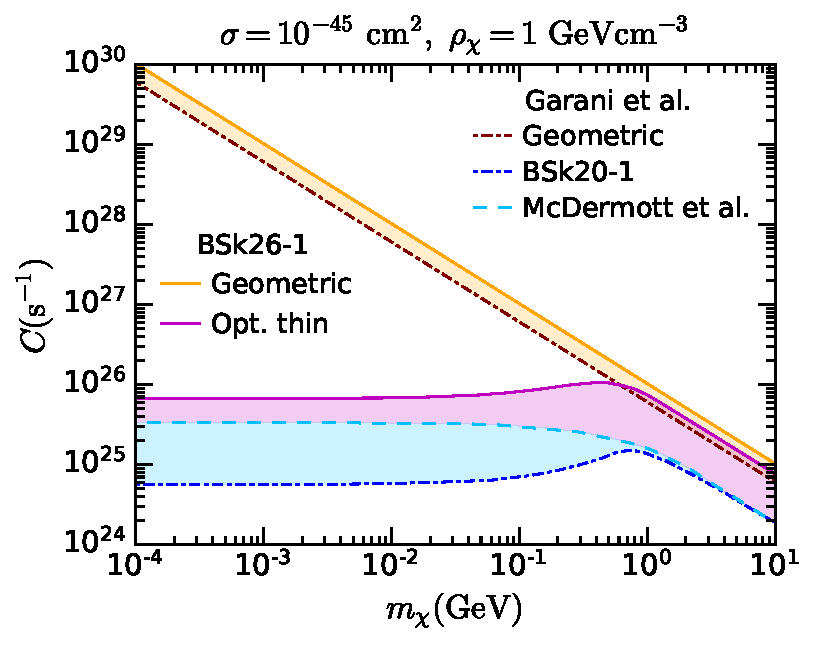
\includegraphics[width=.48\textwidth]{capture_1/capture_rate_n0_comp1.pdf}
    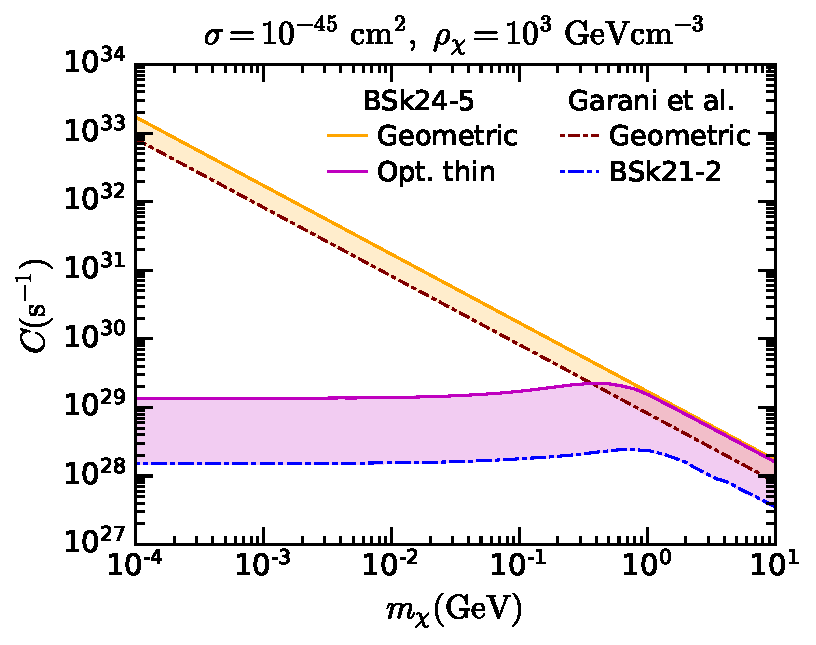
\includegraphics[width=.48\textwidth]{capture_1/capture_rate_n0_comp2.pdf}    
    \caption[Capture rate in the optically thin  (magenta) and geometric (orange) limits as a function of the DM mass for constant cross-section $\sigma=10^{-45}\cm^2$, $\rho_\chi=1\GeV\cm^{-3}$ and BSk26 functional for $\Mstar\simeq1.52\Msun$ and $\Rstar\simeq11.6\km$ denoted as BSk26-1.]{Left: Capture rate in the optically thin  (magenta) and geometric (orange) limits as a function of the DM mass for constant cross-section $\sigma=10^{-45}\cm^2$, $\rho_\chi=1\GeV\cm^{-3}$ and BSk26 functional for $\Mstar\simeq1.52\Msun$ and $\Rstar\simeq11.6\km$ denoted as BSk26-1. Capture rate calculations from Ref.~\cite{Garani:2018kkd_may_NewAnalysisNeutron} for a NS configuration with EoS BSk20-1~\cite{Potekhin:2013qqa_Analyticalrepresentationsunified} equivalent to BSk26-1, are shown for comparison. Right: Same as left but for $\rho_\chi=10^3\GeV\cm^{-3}$ and the benchmark model BSk24-5 equivalent to BSk21-2 in Ref.~\cite{Garani:2018kkd_may_NewAnalysisNeutron}: $\Mstar\simeq2.11\Msun$ and $\Rstar\simeq12.0\km$. 
    }
    \label{ch3:fig:Cratecomp}
\end{figure}
%%%%%%%%%%%%%%%%%%%%%%%%%%%%%%%%%%%%%%%%

%%%%%%%%%%%%%%%%%%%%%%%%%%%%%%%%%%%%%%%%
%%%%%%%%%%%%%%%%%%%%%%%%%%%%%%%%%%%%%%%%
\subsection{Large Mass Regime: Multiple Scattering}
\label{ch3:subsec:largemassandsigma}
%%%%%%%%%%%%%%%%%%%%%%%%%%%%%%%%%%%%%%%%
%%%%%%%%%%%%%%%%%%%%%%%%%%%%%%%%%%%%%%%%


The capture rate expressions obtained in the previous section assume that the cross-section is small enough that the star is in the ``optically thin'' regime, and that a single scatter is sufficient to capture the DM. These assumptions break down if the DM-target cross-section is $\gtrsim\mathcal{O}(\sigmath)$, or if the DM mass exceeds $m_\chi \sim 10^6\GeV$, respectively. 
In this section, we focus on addressing the latter concern as we work in the optically thin regime for the remainder of this work\footnote{The discussion on the effect of the NS opacity in $\sigma\sim \sigmath$ regime can be found in Ref.~\cite{Bell:2020jou_sep_ImprovedTreatmentDark}.}. 
To that end, we now explain how to modify our previous capture rate expressions to account for multiple scattering in a degenerate media\footnote{For a recent discussion on multiple scattering within non-relativistic stars, or with ions in WDs, see Ref.~\cite{Dasgupta:2019juq_Darkmattercapture}.}


In deriving Eq.~\ref{ch3:eq:capturefinal} we had assumed that the DM velocity at infinity, $u_\chi$, can be neglected, such that any interaction where the DM loses energy resulted in its capture. If we instead keep the leading order $u_\chi$ contribution to the total DM energy, the DM energy at infinity is
\begin{equation}
    E^\infty_\chi \sim m_\chi \left(1+\frac{1}{2}u_\chi^2\right), 
\end{equation}
and at a distance $r$ from the star, it gets boosted to
\begin{equation}
    E_\chi(r) = \frac{m_\chi}{\sqrt{B(r)}} \left(1+\frac{1}{2}u_\chi^2\right).
    \label{ch3:eq:Echir}
\end{equation}
Therefore, the amount of energy that the DM must lose to be captured is
\begin{align}
    E_\chi^C(r) & =  \frac{1}{2}u_\chi^2 \frac{m_\chi}{\sqrt{B(r)}}. \\
                & \sim 0.6\GeV \left(\frac{u_\chi}{270\km\s^{-1}}\right)^2 \left(\frac{m_\chi}{10^6\GeV}\right)\left(\frac{0.5}{B(r)}\right)^{1/2}.
\end{align} 
Hence, DM with a mass of $10^6\GeV$ with an initial velocity $u_\chi = 270\km\s^{-1}$, must lose 0.6 GeV of energy for it to be captured. This is of the same order as the maximum amount of energy that can be lost in a single scatter as seen in Fig.~\ref{ch3:fig:q0max}. Given that $\qomax$ plates for $\mchi \gg \mi$, it will be highly improbable that DM heavier than $\sim 10^6\GeV$ loses enough energy in a single scatter to be captured. Single scatter capture is still possible as the DM velocity at infinity is not a fixed value, rather it follows by some distribution function. Therefore, the heavy DM could have a velocity close to zero at infinity, significantly reducing the amount of energy it needs to lose.

To account for this effect, we assume that the DM particles have a speed $u_\chi\ll 1$ at infinity that follows a Maxwell-Boltzmann (MB) distribution, Eq.~\ref{ch3:eq:MB}. 
We can then define the probability density function (PDF) of the energy lost by the DM using the differential interaction rate through
\begin{equation}
\xi(q_0,E_\chi,\kinFi) = \frac{1}{\Gamma^{-}(E_\chi)}\frac{d\Gamma^{-}}{dq_0}(q_0,E_\chi,\kinFi),\label{ch3:eq:normintrate}
\end{equation}
where $\frac{d\Gamma}{dq_0}$ is the DM differential interaction rate, calculated in Appendix~\ref{ch3:sec:diff_int_rate}. 
The function $\xi$ is defined for any $q_0\ge 0$, however, kinematics dicatates that the function is non-zero only for $q_0\le\qomax$. Additionally, note that $\xi$ depends on $B(r)$ through the ratio $E_\chi/m_\chi$, and for brevity we will simply write $\xi(q_0)$.



%%%%%%%%%%%%%%%%%%%%%%%%%%%%%%%%%%
\begin{figure}[t]
    \centering
    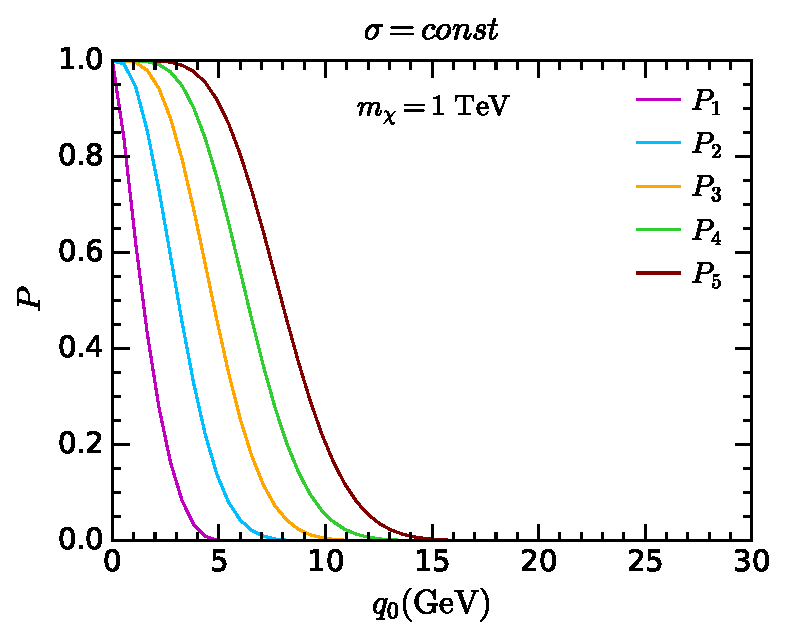
\includegraphics[width=.48\textwidth]{capture_1/probs_n0.pdf}
    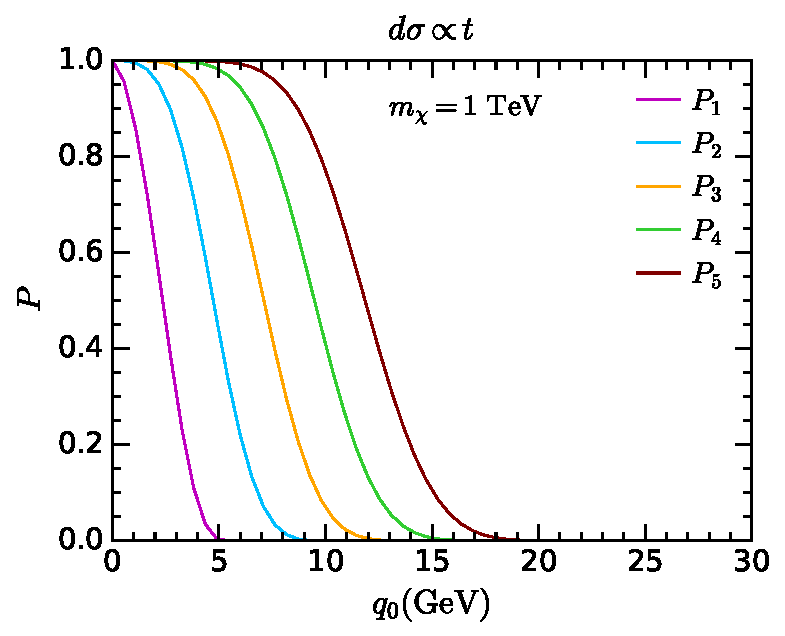
\includegraphics[width=.48\textwidth]{capture_1/probs_n1.pdf}\\
    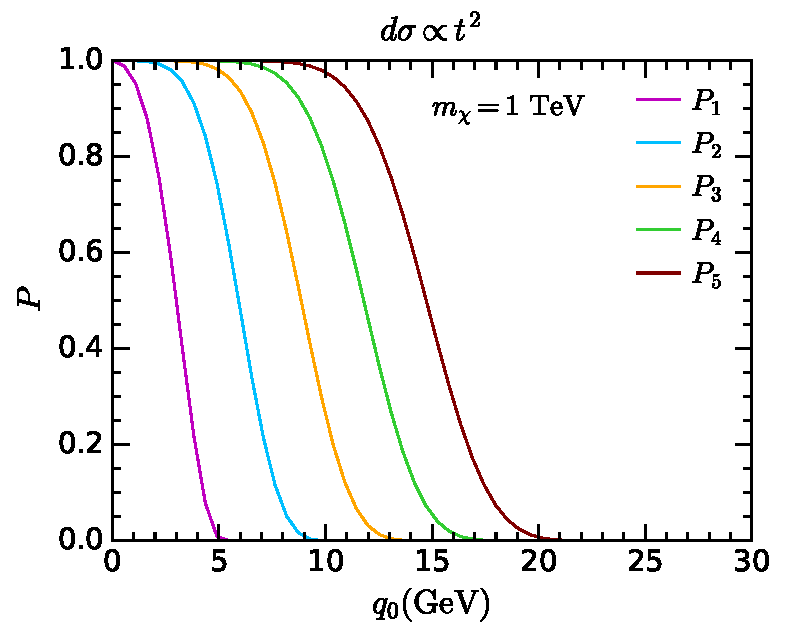
\includegraphics[width=.48\textwidth]{capture_1/probs_n2.pdf}
    \caption[Probabilities to lose at least an amount of energy $\delta q_0$  after $1,...,5$ scatterings,  $P_1,...,P_5$, as a function of the energy loss $q_0$,  assuming $B=0.5$ and $\kinFn=400\MeV$.]{Probabilities to lose at least an amount of energy $\delta q_0$  after $1,...,5$ scatterings,  $P_1,...,P_5$, as a function of the energy loss $q_0$,  assuming $B=0.5$ and $\kinFn=400\MeV$. Results are shown for different dependence on the cross-section on the Mandelstam variable $t$: constant DM-neutron cross-section (top left), $d\sigma\propto t$ (top right) and $d\sigma\propto t^2$ (bottom). }
    \label{ch3:fig:pn}
\end{figure}
%%%%%%%%%%%%%%%%%%%%%%%%%%%%%%%%%%%


We can define the probability of losing at least an amount of energy $q_0 = \delta q_0$ in a single collision as
\begin{equation}
    P_1(\delta q_0) = \int_{\delta q_0}^\infty dx \xi(x).
    \label{ch3:eq:P1}
\end{equation}
The probability of losing at least the same amount of energy after 2 collisions will then be
\begin{align}
 P_2(\delta q_0) &= \int_{\delta q_0}^\infty dy \int_0^\infty dx\;\xi(x) \xi(y-x)\\
    & =  P_1(\delta q_0) + \int_{\delta q_0}^\infty dy \int_0^y dx\; \xi(x)\xi(y-x)\\
    & = P_1(\delta q_0) + \int_0^{\delta q_0} dz \;P_1(\delta q_0-z)\xi(z).
\end{align}
From this, we obtain the following recursive relation for the probabilities, $P_N$, of losing at least $q_0 = \delta q_0$ in $N$ scatters,
\begin{equation}
 P_{N+1}(\delta q_0) = P_N(\delta q_0) + \int_0^{\delta q_0} dz P_N(\delta q_0-z)\xi(z).\label{ch3:eq:pnrecurrent}
\end{equation} 
In Fig.~\ref{ch3:fig:pn} we show how the probability functions $P_1,...,P_5$ changes based on the $t$ dependence of the differential cross-section. We show results for $\sigma=$const. (top left), $d\sigma\propto t$ (top right) and $d\sigma\propto t^2$ (bottom), for fixed values of $B=0.5$, $\kinFn=400\MeV$.

%%%%%%%%%%%%%%%%%%%%%%%%%%%%%%
\begin{figure}
    \centering
    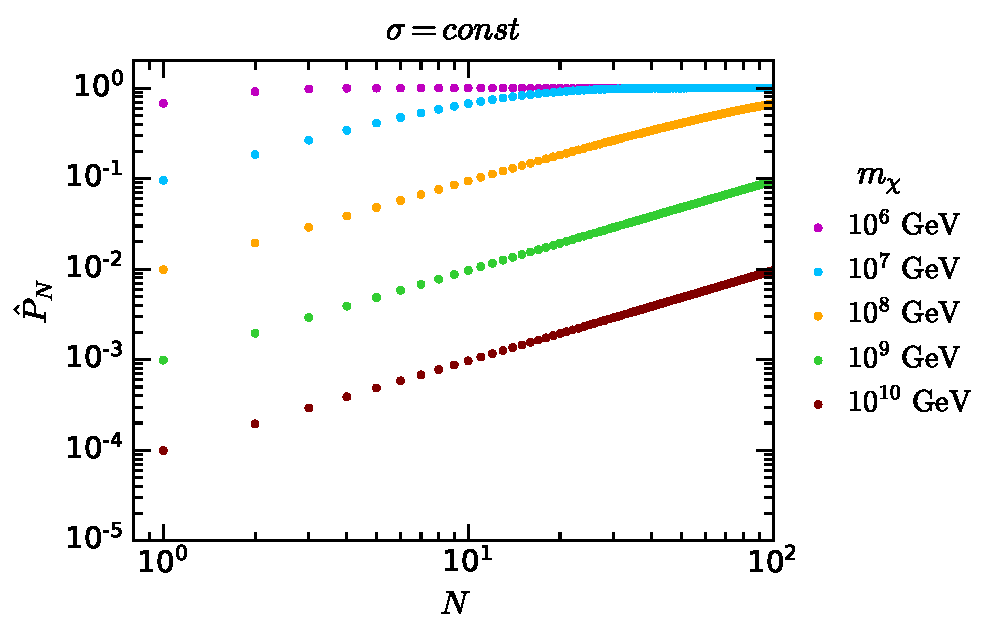
\includegraphics[width=.6\textwidth]{capture_1/cumprobN_n0.pdf}
    \caption[Cumulative probability $\hat{P}_N$ for $B=0.5$,  $\kinFn=400\MeV$ and for $\sigma = \mathrm{const.}$ as a function of the number of scatterings $N$ for several DM masses.]{Cumulative probability $\hat{P}_N$ for $B=0.5$,  $\kinFn=400\MeV$ and for $\sigma = \mathrm{const.}$ as a function of the number of scatterings $N$ for several DM masses.}
    \label{ch3:fig:pnofn}
\end{figure}
%%%%%%%%%%%%%%%%%%%%%%%%%%%%%%

To connect this back to the capture probability, we define the probability for a DM particle to be captured after exactly $N$ interactions, $c_N$, to be $P_N(E^C_\chi) - P_{N-1}(E^C_\chi)$ averaged over the MB distribution of the initial velocity,
\begin{equation}
    \begin{split}
        c_N(r) &= \frac{1}{\int_0^\infty \frac{\fMB(u_\chi)}{u_\chi}du_\chi}\int_0^\infty \frac{\fMB(u_\chi)}{u_\chi}du_\chi \left[P_N\left(\frac{1}{2}\frac{m_\chi u_\chi^2}{\sqrt{B(r)}}\right)\right.\\
        &\hspace{18em}\left. -P_{N-1}\left(\frac{1}{2}\frac{m_\chi u_\chi^2}{\sqrt{B(r)}}\right)\right], 
    \end{split}
\end{equation}
where $c_N$ depends on $r$ through the dependence of $P_N$  on $B(r)$ and $\kinFn(r)$. Note that although our results will assume a Maxwell-Boltzmann velocity distribution, it is straightforward to generalise the results to any other DM velocity distribution. The cumulative probability $\hat{P}_N$ that a DM particle is captured after $N$ interactions with a total energy loss  $\delta q_0=E_\chi^C$ is then
\begin{equation}
\hat{P}_N(r) = \sum_{i=1}^N c_i = \frac{1}{\int_0^\infty \frac{\fMB(u_\chi)}{u_\chi}du_\chi}\int_0^\infty \frac{\fMB(u_\chi)}{u_\chi}du_\chi P_N\left(\frac{1}{2}\frac{m_\chi}{\sqrt{B(r)}} u_\chi^2\right).
\end{equation}
%
The resulting cumulative probability is shown as a function of the number of scatterings $N$ in Fig.~\ref{ch3:fig:pnofn}, for constant cross-section and several DM masses. 

The cumulative probability $\hat{P}_N$ for the above values of $B,\kinFn$ is well approximated by the function\footnote{Further discussion of the multi-scattering regime, and justification of this fitting function, can be found in Appendix~C of Ref.~\cite{Bell:2020jou_sep_ImprovedTreatmentDark}.}
\begin{equation}
\hat{P}_N \sim  1-e^{-\frac{N \mstar}{m_\chi}}.\label{ch3:eq:pncum}
\end{equation}
In particular, the probability that the DM is captured in a single scatter is 
\begin{equation}
c_1=\hat{P}_1 \sim  1-e^{-\frac{\mstar}{m_\chi}}.
\label{ch3:eq:c1}
\end{equation}
From this, we see that $c_1$ will begin to significantly fall below unity for $\mchi \gtrsim \mstar$, and hence multiple scattering will only significantly reduce the capture rate for DM masses above $\mstar$. 

To give an idea for how large the value of $\mstar$ will be, for neutron targets and the values $B=0.5$ and $\kinFn=400$~MeV, we find
\begin{align}
m^{*} &=1.08 \times 10^6 \GeV,\quad \Msq\propto t^0,\\
m^{*} &=1.62 \times 10^6 \GeV,\quad \Msq\propto t^1,\\
m^{*} &=2.01 \times 10^6 \GeV,\quad \Msq\propto t^2.
\end{align}
We illustrate how $m^*_n$ varies with $B$ and $\kinFn$ in Fig.~\ref{ch3:fig:mstarbmu}. 

%%%%%%%%%%%%%%%%%%%%%%%%%%%%%%
\begin{figure}[t!bp]
    \centering
    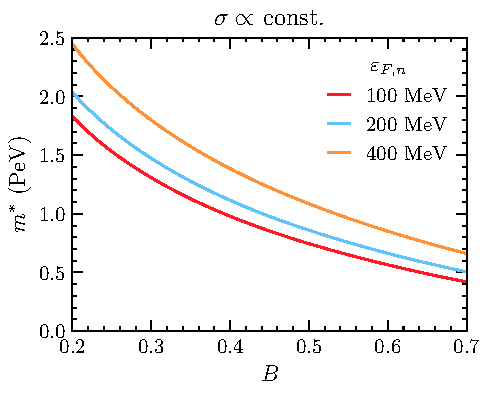
\includegraphics[width=.48\textwidth]{capture_1/mstar_B_n0.pdf}
    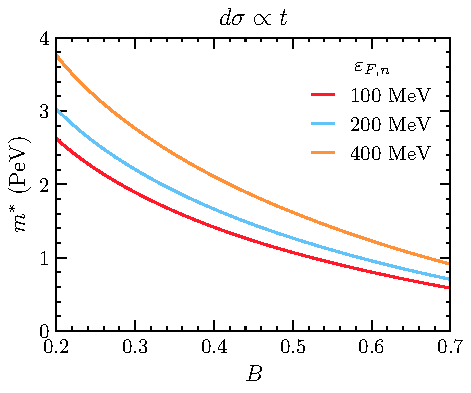
\includegraphics[width=.48\textwidth]{capture_1/mstar_B_n1.pdf}    
    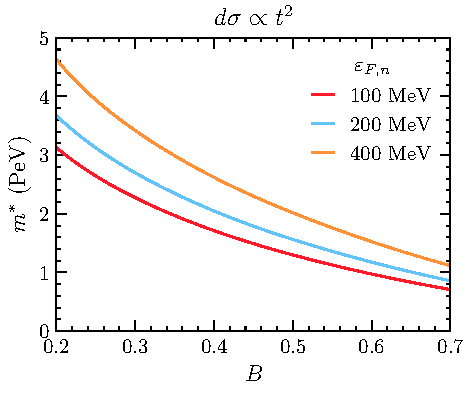
\includegraphics[width=.48\textwidth]{capture_1/mstar_B_n2.pdf}      
    \caption{Value of $m^*_n$ as a function of $B$ for different values of $\kinFn$, $\sigma=const.$ (top left), $d\sigma\propto t$ (top right) and $d\sigma\propto t^2$ (bottom).}
    \label{ch3:fig:mstarbmu}
\end{figure}
%%%%%%%%%%%%%%%%%%%%%%%%%%%%%%

When the cross-section is small, $\sigma\ll\sigmath$, such that we are in the optically thin regime, if the DM does not get captured in its initial scatter, then it will leave the star without interacting again. To account for this, the factor of $c_1$ should be included in the capture rate calculation, Eq.~\ref{ch3:eq:cap_rel_full_1}. However, as we have jsut seen, $c_1\ll1$ only for $\mchi\gtrsim\mstar$, which will always be significantly larger than the target mass and chemical potential. Therefore, multiple scattering is only important in the regime where PB is negligible, and so a suitable approximation for the capture rate in this regime is
\begin{equation}
    C_\mathrm{approx}^* = \frac{4\pi}{\vstar}\frac{\rho_\chi}{m_\chi}{\rm Erf}\left(\sqrt{\frac{3}{2}}\frac{\vstar}{v_d}\right)  \int  r^2 dr  \frac{\sqrt{1-B(r)}}{B(r)}\Omega^{-}(r) c_1(r),
    \label{ch3:eq:capturesimplelargem}
\end{equation}
with $\Omega^-(r)$ calculated as outlined in sections~\ref{ch3:subsec:captureintermediate}
    
% %%%%%%%%%%%%%%%%%%%%%%%%%%%%%%%%%%%%%
% %%%%%%%%%%%%%%%%%%%%%%%%%%%%%%%%%%%%%
\section{Results}
\label{ch3:sec:results}
% %%%%%%%%%%%%%%%%%%%%%%%%%%%%%%%%%%%%%
% %%%%%%%%%%%%%%%%%%%%%%%%%%%%%%%%%%%%%


In this section, we present our results for the capture rate of fermionic DM scattering from neutrons within a NS in the zero temperature approximation. We calculate the capture rate only for scalar/pseudoscalar-scalar/pseudoscalar interactions between DM and neutrons, i.e. effective operators D1-D4 in Table~\ref{ch1:tab:opers_defn_full}, whose differential cross-sections depend only on the Mandelstam variable $t$ and not on $s$. 
We use realistic radial profiles for the neutron number density, chemical potential, and relativistic corrections encoded in $B(r)$ as explained in Section~\ref{ch2:subsec:NS_EoS}, obtained from the BSk24 EoS for the configurations in Table~\ref{ch2:tab:BSk_configs}. 



% Most of our results apply generally to other operators or to other targets (with the mass ranges adjusted appropriately).  Specifically, Eqs.~\ref{eq:captureclsimplrel},~\ref{eq:omegampaulitext}, which are to be evaluated numerically, are applicable to all operators and targets, and work until multiple scattering becomes relevant, when $m_\chi\gtrsim \qomax/v_{\star}^2$.
% The optical factor of Eq.~\ref{eq:optfactor} for the intermediate mass range is also applicable to all operators and targets. The optical factor of Eq.~\ref{eq:optfactorlargem} and the value of $m^*$, which are used to include multiple scattering effects in the large mass range, $m_\chi\gtrsim \qomax/v_{\star}^2$, can be easily computed for operators D1-D4 (or any other operator that depends only on $t$) for all targets. For other operators it can be used only by numerically solving the shape of the differential rate, a task that may be computationally intensive to achieve with high precision.
% Our approximated formulas, Eqs.~\ref{eq:csimplelargemtext},~\ref{eq:capturesimplelargem} and \ref{eq:captureopticaldepth} have been checked to be accurate only for nucleon targets, but can be applied to any operator (for $s$-dependent ones, see Appendix~\ref{sec:capratesimple} on how to remove the $s$ dependence). In any case, one can substitute the relevant factors ($\eta,m^*$) into Eqs.~\ref{eq:captureclsimplrel},~\ref{eq:omegampaulitext} to calculate the capture rate, in the appropriate mass range, for other targets.




To estimate the NS EoS impact on the DM capture rate computation, we numerically calculate $C$ using the exact expression in the optically thin limit, Eq.~\ref{ch3:eq:capturefinalM2}, that properly accounts for gravitational focusing and Pauli blocking.  In the optically thin regime that we are working in, the capture rate is proportional to the differential DM-neutron cross-section. 
Fig.~\ref{ch3:fig:captureEOS} shows how this rate varies with the NS  EoS for operators D1-D4 and the EoS configurations given in Table~\ref{ch2:tab:BSk_configs}, and in turn with the NS mass and radius. 
The cross-section is normalised such that the capture rate in the intermediate mass range, which is unaffected by PB and multiple scattering, is equal to the geometric limit. It is worth remarking that cross-sections larger than the threshold cross-section should not be used in the optically thin limit, as this would result in capture rates larger than the geometric limit. To account for such large cross-sections, the optical depth of the NS must be accounted for as prescribed in Ref.~\cite{Bell:2020jou_sep_ImprovedTreatmentDark}.
Depending on the operator considered, going from the lightest to the heaviest NS can change the capture rate by a minimum of one order of magnitude, such as in the case of operators D1, D2 and D3 (at low DM mass), and up to 2 orders of magnitude, as in the case of operators D2 for large DM mass, and D4 in general. 

%%%%%%%%%%%%%%%%%%%%%%%%%%%%%%
\begin{figure}[t!bp]
    \centering
    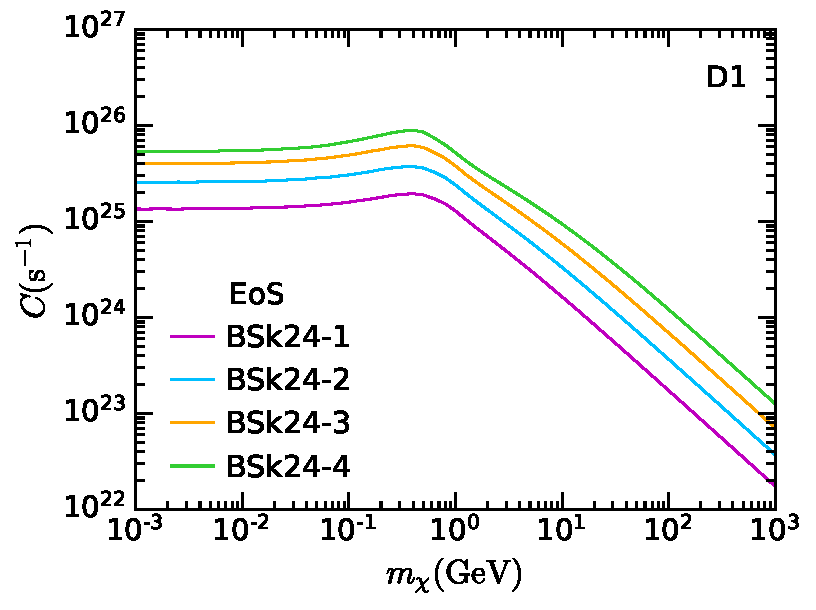
\includegraphics[width=.45\textwidth]{capture_1/capture_rate_numeric_EOS_D1.pdf}
    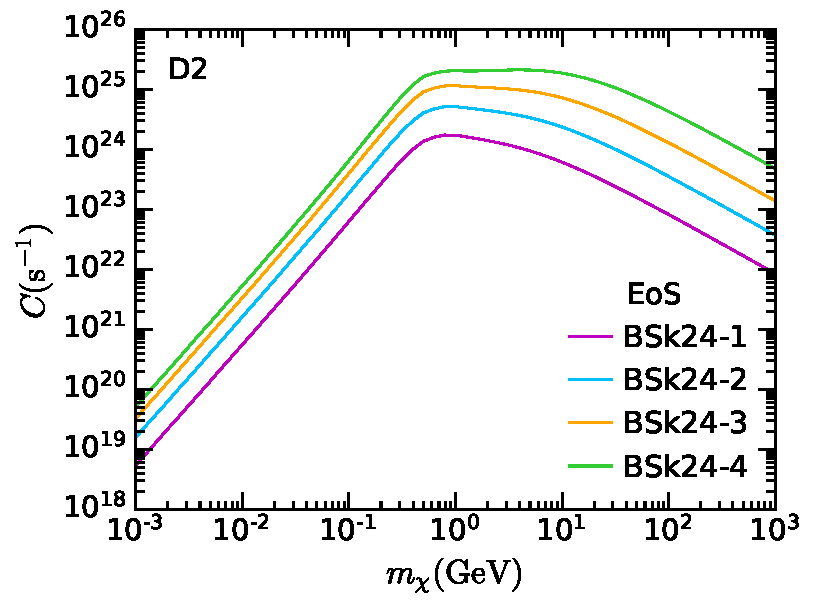
\includegraphics[width=.45\textwidth]{capture_1/capture_rate_numeric_EOS_D2.pdf}\\
    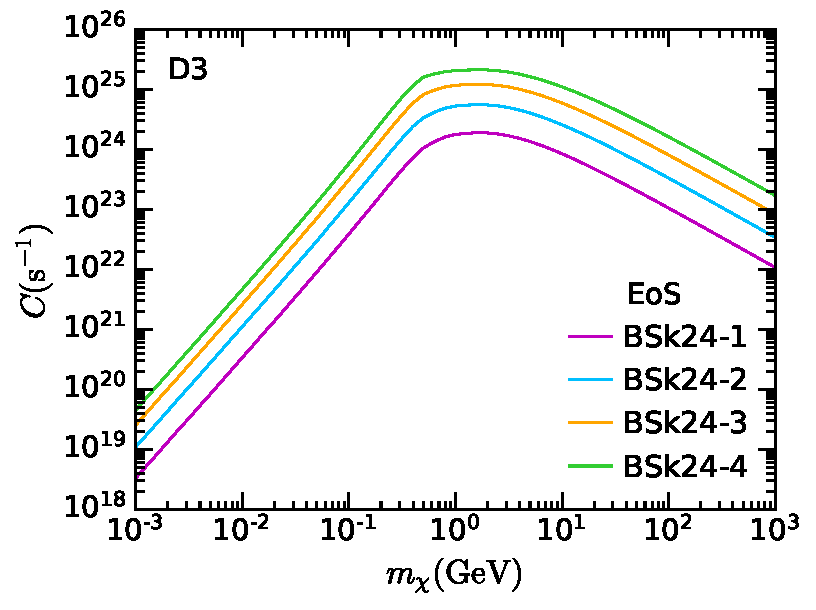
\includegraphics[width=.45\textwidth]{capture_1/capture_rate_numeric_EOS_D3.pdf}
    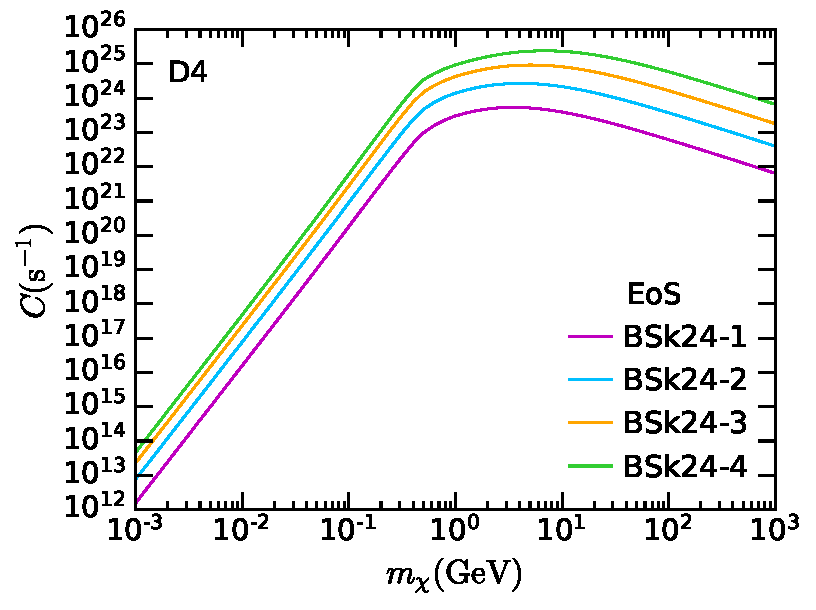
\includegraphics[width=.45\textwidth]{capture_1/capture_rate_numeric_EOS_D4.pdf}
    \caption[Capture rate in the optically thin limit as a function of the DM mass for $\sigma=\sigmaref\sim 1.7 \times 10^{-45} \cm^2$ and the configurations of the EoS BSk24 given in Table~\ref{ch2:tab:BSk_configs}.]{Capture rate in the optically thin limit as a function of the DM mass for $\sigma=\sigmaref\sim 1.7 \times 10^{-45} \cm^2$ and the configurations of the EoS BSk24 given in Table~\ref{ch2:tab:BSk_configs}. Rate calculated using the 4-dimensional integral in Eq.~\ref{ch3:eq:capturefinalM2}, that includes Pauli blocking but neglects the NS opacity and multiple scattering. Results are shown for the EFT operators D1 (top left), D2 (top right), D3 (bottom left) and D4 (bottom right) in Table~\ref{ch1:tab:opers_defn_full}.}
    \label{ch3:fig:captureEOS}
\end{figure}
%%%%%%%%%%%%%%%%%%%%%%%%%%%%%%




At large DM mass, all operators show the same scaling with the DM mass. At  $m_\chi\lesssim1\GeV$, a different picture arises as Pauli blocking leads to different suppressions of the capture rate for the different operators. However, we observe that the four operators give very similar results to those of Fig.~\ref{ch3:fig:approxc}, where we analysed the dependence of the capture rate on the momentum transfer $t$.  We note that operator D1, which contains in its squared matrix element a term independent of $t$, gives a result that is very similar to that of $\sigma=\mathrm{const}$. Operators D2 and D3, for which $\Msq$ does not include terms independent of $t$, but rather terms proportional to $t$ and $t^2$, yield very similar results to that of $d\sigma\propto t$. 
Overall, we conclude that the lowest power of the transferred momentum determines the mass scaling of the capture rate at low DM  mass.
This result holds true for matrix elements that depend also on $s$. 


%%%%%%%%%%%%%%%%%%%%%%%%%%%%%%
\begin{figure}[t!bp]
    \centering
    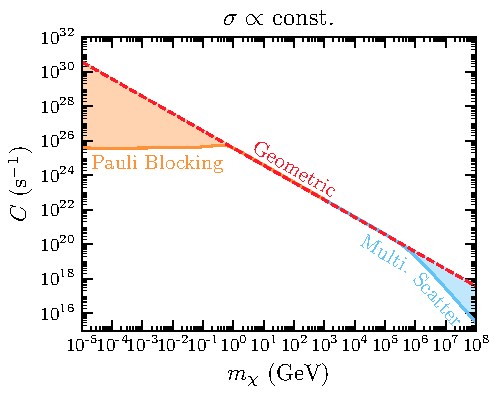
\includegraphics[width=.48\textwidth]{capture_1/capture_rate_n0_fullmassrange.pdf}    
    % 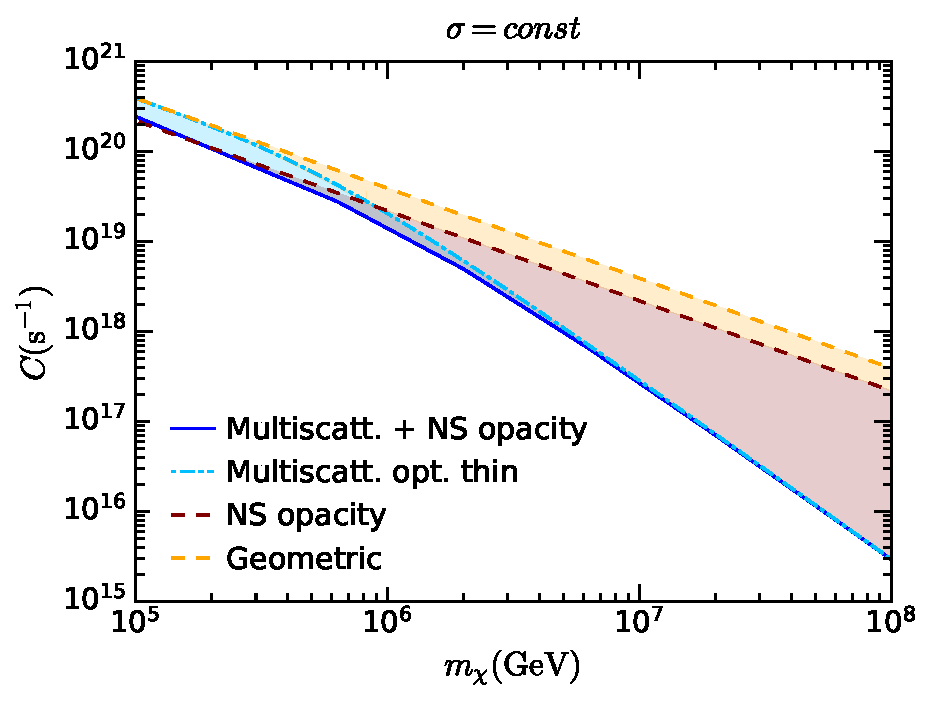
\includegraphics[width=.48\textwidth]{capture_1/capture_rate_n0_largemass.pdf} %\\
    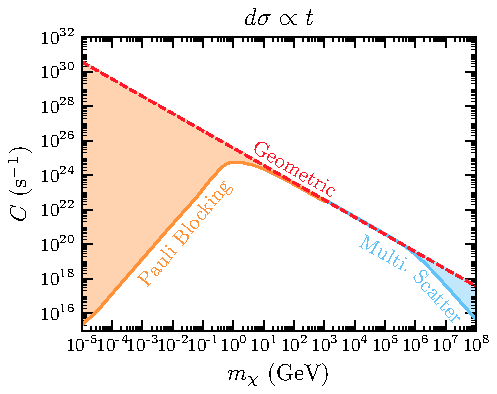
\includegraphics[width=.48\textwidth]{capture_1/capture_rate_n1_fullmassrange.pdf}       
    % 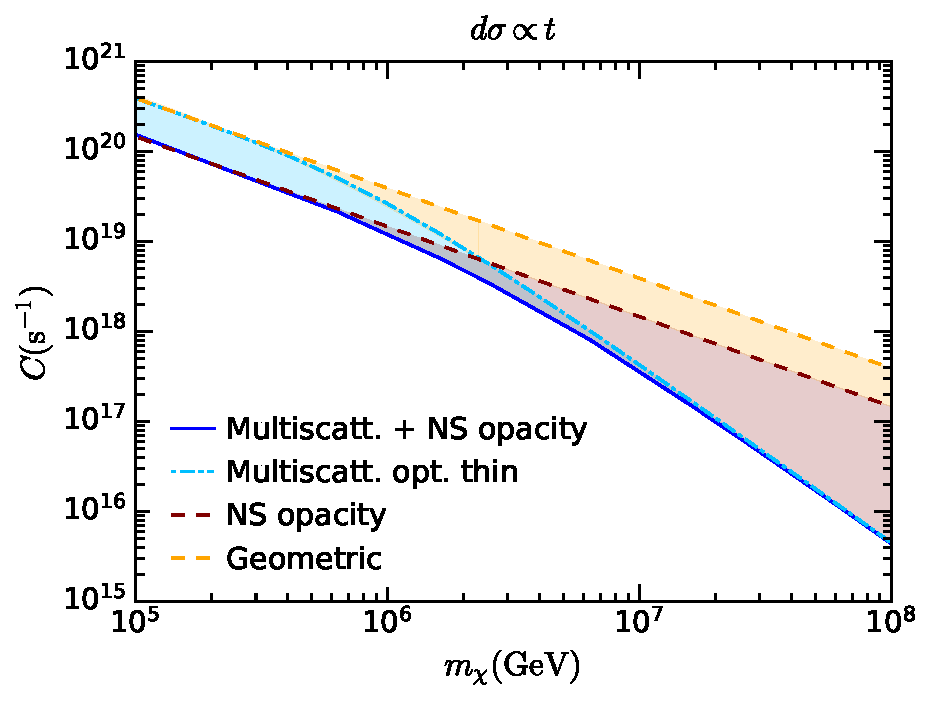
\includegraphics[width=.48\textwidth]{capture_1/capture_rate_n1_largemass.pdf} \\
    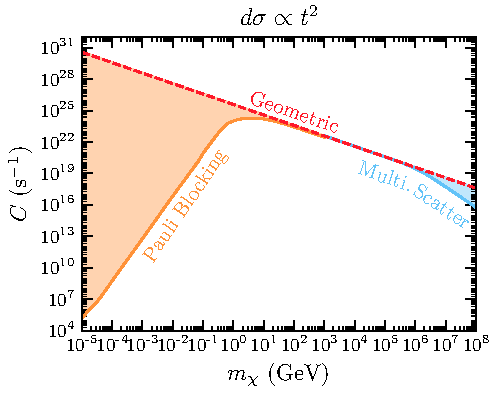
\includegraphics[width=.48\textwidth]{capture_1/capture_rate_n2_fullmassrange.pdf}       
    % 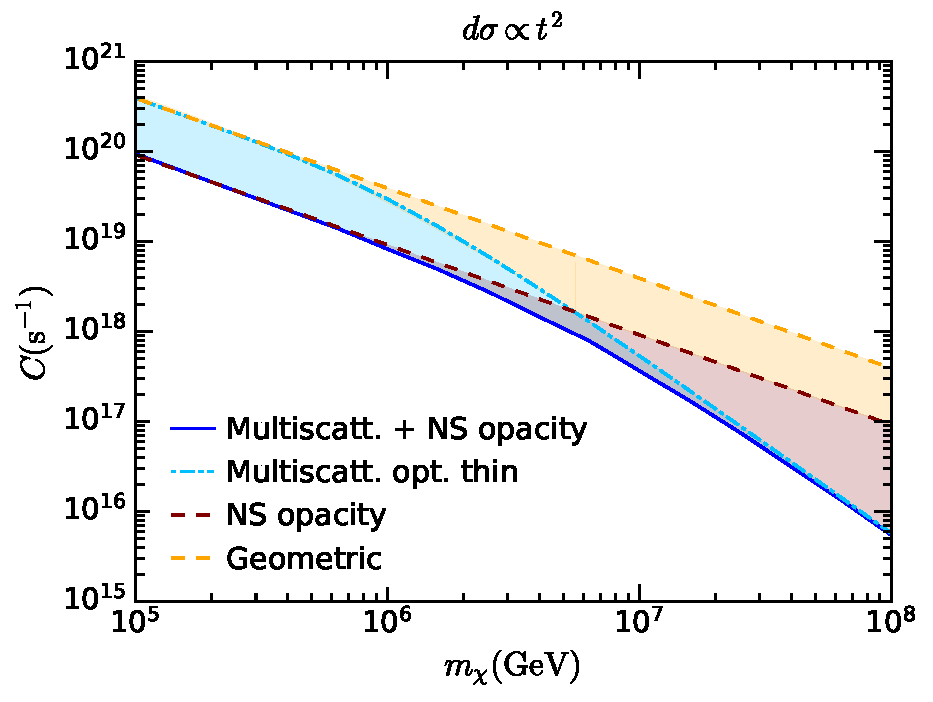
\includegraphics[width=.48\textwidth]{capture_1/capture_rate_n2_largemass.pdf}        
    \caption[Capture rate for constant cross-section (top left), $d\sigma\propto t$ (top right) and $d\sigma\propto t^2$ (bottom),  for  $\sigma=\sigmaref\sim 1.7 \times 10^{-45}\cm^2$ and NS EoS configuration BSk24-2.]{Capture rate for constant cross-section (top left), $d\sigma\propto t$ (top right) and $d\sigma\propto t^2$ (bottom),  for  $\sigma=\sigmaref\sim 1.7 \times 10^{-45}\cm^2$ and NS EoS configuration BSk24-2. These plots extent the mass range of those in Fig.~\ref{ch3:fig:approxc} to large DM masses.
    }
    \label{ch3:fig:capturelargemass}
\end{figure}
%%%%%%%%%%%%%%%%%%%%%%%%%%%%%%

In Fig.~\ref{ch3:fig:capturelargemass}, we show the capture rate for a broad DM mass range, spanning 13 orders of magnitude from $m_\chi=10\keV$ to $m_\chi=10^8\GeV$, including all three of the mass regimes we have discussed in the previous sections, for $d\sigma\propto const.$ (first row), $t^1$ (second row) and $t^2$ (third row).
The orange line indicates the capture rate calculated in the optically thin limit using the 4-dimensional integration in Eq.~\ref{ch3:eq:capturefinal} that accounts for Pauli blocking. 
At large DM masses, Pauli suppression plays no role and the capture rate approaches the geometric limit (dashed red line). 
We also show in Fig.~\ref{ch3:fig:capturelargemass} the effect of the inclusion of multiple scattering in the light blue line, which becomes relevant at $m_\chi\sim10^6\GeV$. 
% The difference among these calculations is better shown in the right panels, where only the large DM mass range is considered. The brown dashed line indicates the result that includes the optical depth factor $\eta$ but neglects multiple scattering, obtained using Eq.~\ref{eq:optfactor} in Eq.~\ref{eq:captureopticaldepth}.   
% As we can see, for $\sigma=\sigmaref$ this causes a small suppression of the capture rate, when compared to the result where the optical depth factor is ignored (light blue dot dashed line). For larger $\sigma$, neglecting the optical depth would result in a capture rate that exceeds the geometric limit (orange dashed line), while the inclusion of the optical depth factor $\eta$ causes the capture rate to saturate, tending to  $C_{geom}$ for large cross-sections. 
% The light blue dot dashed line indicates the capture rate calculated by neglecting the optical depth factor, but including multiple scattering, given by Eq.~\ref{eq:capturesimplelargem}. 
At $m_\chi\sim 10^5\GeV$ that line matches the geometric limit as expected from the chosen value of the cross-section $\sigma=\sigmaref$. At larger DM masses, $m_\chi\gtrsim10^6\GeV$, multiple scatterings are required for the DM to be captured, hence an additional suppression factor of $1/m_\chi$ arises, as given in Eq.~\ref{ch3:eq:capturesimplelargem}. Therefore, the capture rate becomes increasingly smaller than $C_{geom}$ (light blue shaded area). 
% Finally, the capture rate calculated including both effects is depicted in blue. At $m_\chi\sim10^5\GeV$, we can observe the suppression produced by the optical depth factor $\eta$ (light blue shaded region), while at larger DM masses the proper additional suppression $1/m_\chi$ emerges. 

Comparing the plots for different $t^n$ dependence, we can see that increasing the power of $n$ has a small effect on the mass scale where the various suppressions become relevant. For example, comparing the light blue lines between the three figures, we see that the change of slope from the onset of multiple scattering moves slightly further to the right for larger $n$. This is a consequence of the fact that larger powers of $n$ result in larger energy transfer (see, for example, Fig.~\ref{app:fig:diffgamma}), leading to a larger capture probability $c_1$ and hence a larger $\mstar$.
However, the qualitative behaviour is the same for all choices of $d\sigma$: the suppression of the capture rate is primarily due to Pauli blocking at low mass and multiple scattering effects (i.e. a low capture probability) at large masses.


%%%%%%%%%%%%%%%%%%%%%%%%%%%%%%%%%%
%%%%%%%%%%%%%%%%%%%%%%%%%%%%%%%%%%
\section{Summary}
\label{ch3:sec:conclusion}
%%%%%%%%%%%%%%%%%%%%%%%%%%%%%%%%%%
%%%%%%%%%%%%%%%%%%%%%%%%%%%%%%%%%%


In this chapter, we have improved and extended the existing framework used to calculate the DM capture rate in the Sun to be compatible with compact objects, relaxing the simplifying assumptions that have previously been made. Specifically, we have derived exact expressions for the capture rate that correctly incorporate relativistic kinematics, gravitational focusing, Pauli blocking, and multiple-scattering effects. We also properly incorporate the internal structure of the star, consistently calculating the radial profiles of the EoS-dependent parameters and the general relativistic corrections, by solving the Tolman-Oppenheimer-Volkoff equations.

This new formalism was applied to neutron stars to highlight the features of the formalism mentioned above.
Neutron stars (and compact objects in general) are composed of strongly degenerate matter, resulting in significant Pauli blocking of scattering interactions when the dark matter is light, $m_\chi\lesssim \mi$, suppressing the capture rate by several orders of magnitude. By including the radial dependence of the chemical potential in our calculations, we correctly account for Pauli suppression at any point in the star. However, note that the chemical potential is dependent on the EoS assumption.


For very large DM masses, $m_\chi\gtrsim10^6\GeV$, the energy lost in a single collision will be insufficient for it to be captured. Hence, the DM must scatter multiple times within an orbit to be captured, or else it simply leaves the star. To correctly compute the DM capture probability due to multiple scattering, we have derived, for the first time, an exact equation for the DM interaction rate in degenerate matter, and used that result to compute the differential capture rate as a function of the DM energy loss. This enables us to compute the cumulative probability that a DM particle is captured after multiple interactions, by averaging over the initial DM velocity distribution.


Although we have framed our results in terms of the scattering of DM from neutron targets in neutron star, it is straightforward to obtain the capture rate for DM scattering from any other degenerate species in compact objects. In the next chapter, we apply this formalism to DM scattering off the leptonic compoennts of NSs, as well as the degenerate electrons within WDs.
